\documentclass[a4paper,12pt]{article}

\usepackage[left=25mm, right=25mm, top=25mm, bottom=25mm]{geometry}

\usepackage{amsmath}
\usepackage{amssymb}
\usepackage{amsfonts}
\usepackage[style=iso]{datetime2}
\usepackage[explicit]{titlesec}
\usepackage{amsthm}
\usepackage{mathrsfs}
\usepackage{array}
\usepackage{graphicx}
\usepackage{mathtools} % Provides \mathrlap command
\usepackage{xparse}
\usepackage{float}
\usepackage{fixdif}
\usepackage[skip=1em,indent]{parskip}
\usepackage{caption}
\usepackage{tocloft}
\usepackage{enumitem}
\usepackage{xurl}
\usepackage[toc, page]{appendix}
\usepackage{accents}
\usepackage[perpage, symbol*]{footmisc} % for dagger footnotes
\DefineFNsymbols{sym}{\textdagger \textdaggerdbl \textsection \textparagraph %
{\textdagger\textdagger} {\textdaggerdbl\textdaggerdbl} %
{\textsection\textsection} {\textparagraph\textparagraph}}
\setfnsymbol{sym}
\interfootnotelinepenalty=10000

\usepackage{tikz}
\usepackage{tikz-3dplot}
\tikzset{>=latex} % for LaTeX arrow head
\usepackage{pgfplots} % for the axis environment
\usetikzlibrary{calc,decorations.markings,external}
\tikzexternalize[prefix=tikz/]

\pgfplotsset{compat=1.18, every tick label/.append style={font=\footnotesize}}

\graphicspath{ {./Images/} }

\usepackage[backend=biber, style=numeric, sorting=none]{biblatex}
\addbibresource{motivational_differential_forms_intro.bib}

\setcounter{biburlnumpenalty}{9000}
\setcounter{biburlucpenalty}{9000}
\setcounter{biburllcpenalty}{9000}

\usepackage[T1]{fontenc}
\usepackage{microtype, mlmodern}
\usepackage[bb=ncmbbk, bfbb]{mathalpha}

% ---------------- %
\usepackage{etoolbox}
\usepackage[dvipsnames]{xcolor}
\usepackage[linkcolor=black]{hyperref}
\usepackage[nameinlink]{cleveref}

% Configure cleveref for appendix sections and figures
\crefname{appsec}{Appendix}{appendices}
\Crefname{appsec}{Appendix}{Appendices}
\crefname{figure}{Figure}{Figures}
\Crefname{figure}{Figure}{Figures}


\definecolor{RoyalRed}{RGB}{155, 28, 49}
\definecolor{RoyalOrange}{RGB}{249, 146, 69}
\definecolor{PigmentBlue}{RGB}{51,51,153}

\makeatletter %* Creates a footnote colour option
\def\@footnotecolor{black}
\define@key{Hyp}{footnotecolor}{%
 \HyColor@HyperrefColor{#1}\@footnotecolor%
}
\patchcmd{\@footnotemark}{\hyper@linkstart{link}}{\hyper@linkstart{footnote}}{}{}
\makeatother

\hypersetup{
  colorlinks = true,
  linkcolor = PigmentBlue,
  urlcolor = RoyalRed,
  citecolor = RoyalOrange,
  footnotecolor = black,
}
% ---------------- %
\makeatletter
\def\th@plain{%
  \thm@notefont{}% same as heading font
  \itshape % body font
}
\def\th@definition{%
  \thm@notefont{}% same as heading font
  \normalfont % body font
}
\makeatother

\newcommand*\diff{\mathop{}\!d} % for the differential in integrals
% ---------------- %
\ExplSyntaxOn %* This command is for row vectors; unstarred version has no delimiter scaling for inline; starred version has delimiter scaling for display
\seq_new:N \l_user_rvec_seq

% expl3 worker (does the splitting/formatting)
\cs_new_protected:Npn \dbacc_rvec:n #1
 {
  \seq_clear:N \l_user_rvec_seq
  \seq_set_split:Nnn \l_user_rvec_seq { , } { #1 }
  \seq_use:Nn \l_user_rvec_seq { \enspace }
 }

% plain-name wrapper (no ':' in its name) — safe to call outside ExplSyntaxOn
\cs_new_protected:Npn \dbaccrvec #1 { \dbacc_rvec:n { #1 } }

% user-level \rvec interface (star + optional size + mandatory arg)
\NewDocumentCommand \rvec { s o m }
 {
  \IfBooleanTF{#1}
    { \left[\,\dbaccrvec{#3}\,\right] } % starred -> automatic \left...\right
    { \IfValueTF{#2}
        { \mathopen{#2[}\,\dbaccrvec{#3}\,\mathclose{#2]} } % sized optional arg
        { [\,\dbaccrvec{#3}\,] } % default small delimiters
    }
 }
\ExplSyntaxOff
% ---------------- %
\newcommand{\R}{\mathbb{R}}
\newcommand{\C}{\mathbb{C}}
\newcommand{\Z}{\mathbb{Z}}

\NewCommandCopy{\oldIm}{\Im}
\renewcommand{\Im}{\mathop{\oldIm\mathfrak{m}}}
\NewCommandCopy{\oldRe}{\Re}
\renewcommand{\Re}{\mathop{\oldRe\mathfrak{e}}}

\newcommand{\overbar}[1]{\mkern 1.5mu\overline{\mkern-1.5mu#1\mkern-1.5mu}\mkern 1.5mu}

\DeclareMathOperator{\Res}{Res}

\DeclarePairedDelimiterX{\norm}[1]{\lVert}{\rVert}{#1}
\DeclarePairedDelimiterX{\abs}[1]{\lvert}{\rvert}{#1}
\NewDocumentCommand{\eval}{s m m g}{%
  \IfBooleanTF{#1}
    {% starred version - no scaling
      #2 \vert%
      _{#3}%
      \IfNoValueTF{#4}{}{^{#4}}%
    }
    {% unstarred version - auto-scaled
      \left. #2 \right|%
      _{#3}%
      \IfNoValueTF{#4}{}{^{#4}}%
    }%
}

\makeatletter
\NewDocumentCommand{\extp}{e{^}}{%
  \mathop{\mathpalette\extp@{#1}}\nolimits
}
\NewDocumentCommand{\extp@}{mm}{%
  \textstyle\bigwedge\nolimits\IfValueT{#2}{^{\extp@@{#1}#2}}%
  \IfValueT{#1}{\kern-2\scriptspace\nonscript\kern2\scriptspace}%
}
\newcommand{\extp@@}[1]{%
  \mkern
    \ifx#1\displaystyle-1\else
    \ifx#1\textstyle-1\else
    \ifx#1\scriptstyle-1\else
    -0.5\fi\fi\fi
  \thinmuskip
}
\makeatletter
% ---------------- %
\newcommand{\ihat}{\boldsymbol{\hat{\imath}}}
\newcommand{\jhat}{\boldsymbol{\hat{\jmath}}}
\newcommand{\khat}{\boldsymbol{\hat{k}}}
\newcommand{\ehat}{\mathbf{\hat{e}}}
\newcommand{\T}{\mathrm{T}}
% ---------------- %

\newtheorem{theorem}{Theorem}
\newtheorem{lemma}[theorem]{Lemma}
\newtheorem{proposition}[theorem]{Proposition}
\newtheorem{corollary}{Corollary}[theorem]

\theoremstyle{definition}
\newtheorem{definition}[theorem]{Definition}
\newtheorem{example}[theorem]{Example}

% \setlength{\cftsecnumwidth}{3em}

\begin{titlepage}
\title{A Motivational Introduction to Differential Forms}
\author{Abdul Musthakin}
\date{January 2026}
\end{titlepage}

% \renewcommand{\thesection}{\Roman{section}}

\allowdisplaybreaks

\setlength{\parindent}{0pt}

\begin{document}
\maketitle

\pagebreak

\tableofcontents

\pagebreak

\section*{Prerequisites}

This exposition aims to require as little prerequisite knowledge as possible in order for one to be able to understand the presented concepts.
However, there are still some topics that are absolutely essential.
This includes concepts in single and multivariable calculus, as well as introductory linear algebra.
The rigorous underpinnings of these topics, such as the contents of a course on real analysis, are not required.
If relevant, they will be attached as an appendix.

\subsection*{1. Linear Algebra}
Expertise in linear algebra is by no means necessary.
A surface-level understanding of the main ideas should suffice:
\begin{itemize}
    \item The intuitive idea of vectors as ordered lists of numbers or arrows in a plane.
    \item Elements of $\R^n$ as vectors.
    \item The concept of matrices being linear maps and representing transformations, as well as basic ideas relating to them (linear maps in general are important).
    \item Vector operations: dot (scalar) product, inner product, cross product.
    \item Matrix multiplication, determinants, transpose, and inverse of matrix.
    \item The idea of vectors being more general objects (elements of a vector space).
    \item The basis and dimension of a vector space, and the concept of vector subspaces.
\end{itemize}
Besides general knowledge of vectors and linear algebra, the most important concept here to be aware of is that vectors are much more general than coordinates and arrows.
We will encounter objects that are vectors but are completely different from the aforementioned `typical' examples.
See \cref{appendix:vector_space} for the definition of a vector space, but note that this is only intended to be a reference.

\subsection*{2. Multivariable Calculus}
Knowledge of some concepts in multivariable calculus is mandatory.
Single-variable calculus is obviously a requirement by extension.
Whilst the topic of differential geometry -- where differential forms are usually found -- is quite a bit more advanced, this introductory exposition is supposed to be a natural part or extension to the concepts of multivariable calculus.
Thus, full familiarity with the subject is not required; many ideas will be developed along the way.
It assumed that one is aware of:
\begin{itemize}
    \item functions of the type $\mathbb{R}^n \to \mathbb{R}^m$;
    \item partial derivatives and the chain rule;
    \item directional derivatives and their computation;
    \item the intuitive ideas behind gradients, divergence, and curl, as well as how to compute them; and
    \item the Jacobian matrix of a multivariable function.
\end{itemize}
A formal introduction to vector calculus is presented in \cref{appendix:vector calculus}.
This will include the definition of the limit of vector-valued functions and the derivation of the Jacobian matrix.
Knowledge of some concepts from real analysis is required to understand this, but they are not required for the main body of the exposition.
The more experience one has with multivariable calculus, the easier it will be for them to understand this exposition.
Just as importantly, it will better enable us to appreciate the value of what is to be introduced.

The last point holds true for any other topic in maths that may be related to differential forms.
This comes both from the perspective of acquiring more knowledge, and gaining experience and maturity.
For instance, abstract algebra (e.g. group theory) is specifically not a prerequisite.
However, knowledge of concepts from it will frequently be useful.
These concepts are intuitive, so they can be mentioned whenever in an informal manner, avoiding the associated jargon.
We encounter isomorphisms between spaces, describing them as associating objects in a specific way, and so on.

\pagebreak

\section{Introduction \& Motivation}

Understanding what an integral means, in a general sense, is not particularly difficult.
Given a function, it is pretty easy to draw it as a curve on a graph.
By looking at its graph and choosing some interval on the $x$-axis, we can see the area between the curve and the $x$-axis.
This (signed) area is what is calculated by an integral.

\begin{figure}[!htbp]
\centering
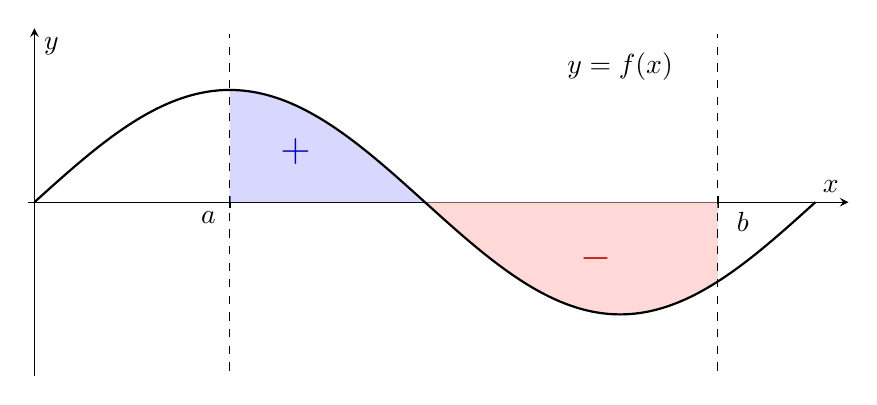
\begin{tikzpicture}
\begin{axis}[
    width=12cm,
    height=6cm,
    axis lines=middle,
    xlabel={$x$},
    ylabel={$y$},
    xmin=0, xmax=6.5,
    ymin=-1.5, ymax=1.5,
    xtick={1.5708, 5.49779},
    xticklabels={},
    ytick=\empty,
    samples=200,
    domain=0:2*pi,
    enlargelimits={abs=0.05},
    tick style={black, thick},
    major tick length=0.15cm,
]

% Labels for a and b
\node[below] at (axis cs:1.4, 0) {$a$};
\node[below] at (axis cs:5.7, 0) {$b$};

% Shaded area for positive region (a to π)
\addplot[fill=blue!30, opacity=0.5, domain=1.5708:3.14159, draw=none] 
    {sin(deg(x))} \closedcycle;

% Shaded area for negative region (π to b)
\addplot[fill=red!30, opacity=0.5, domain=3.14159:5.49779, draw=none] 
    {sin(deg(x))} \closedcycle;

% The sin(x) function
\addplot[black, thick, domain=0:2*pi] {sin(deg(x))};

% Vertical lines at x=a and x=b
\addplot[dashed, black] coordinates {(1.5708, -1.5) (1.5708, 1.5)};
\addplot[dashed, black] coordinates {(5.49779, -1.5) (5.49779, 1.5)};

% Label for the function
\node[above, black] at (axis cs:4.71239, 1) {$y = f(x)$};

% Labels for areas
\node[blue!70!black, font=\Large] at (axis cs:2.1, 0.45) {$+$};
\node[red!70!black, font=\Large] at (axis cs:4.52, -0.5) {$-$};

\end{axis}
\end{tikzpicture}
\caption{A definite integral}
\label{fig:definite_integral_sin}
\end{figure}

The area illustrated by the above figure is given by
\begin{equation*}
    \int_{a}^{b} f(x) \diff x.
\end{equation*}
Now, everything that was just stated has many asterisks.
We can have functions that cannot be integrated, or at least, not in the `usual' sense.
Even if we can integrate a function, we might not be able to get our integral (and thus desired area) in terms of functions that we are used to.
Even if we ignore all of that, there is plenty of theory regarding how we define integrals -- extending and generalizing to different applications.
So it turns out that integrals are not that simple, but their idea is.

The above refers specifically to definite integrals, and so too will further discussion.
It would thus be useful to have a brief mention of indefinite integrals for the sake of completeness.
An indefinite integral of some function $f$ is itself not a number, nor even a function.
It is a class of functions,\footnote{An equivalence class.} whose shared property is that their derivative is $f$.
A member of this class is referred to as an antiderivative of $f$, and it can be written as
\begin{equation*}
    F(x) \coloneq c + \int_{a}^{x} f(t) \diff t,
\end{equation*}
where $a$ and $c$ are some constants.
Since any antiderivative (and thus the indefinite integral) of a function can be rewritten in terms of a definite integral, there is nothing regarding the former concept that warrants its mention in the discussions ahead.

Consider the notation we use for integrals.
We have a unique symbol, $\int$, to always know when we are integrating.
We have the integrand after that, which is what we are integrating.
Also, we have the start and end points of our interval which we are integrating over.
Finally, we have something on the end.
It is definitely not useless, as it tells us what variable we are integrating with respect to.
For instance, it is true that
\begin{equation*}
    \int_{a}^{b} f(x) \diff x = \int_{a}^{b} f(t) \diff t = \int_{a}^{b} f(u) \diff u,
\end{equation*}
just as it is true that
\begin{equation*}
    \sum_{i=1}^{n} f(i) = \sum_{j=1}^{n} f(j) = \sum_{k=1}^{n} f(k).
\end{equation*}
The exact symbol we use for the variable does not matter; they are just labels for the same thing.
Now, in the context of sums, one can simply expand out to show that they are the same thing.
They all refer to $f(1) + f(2) + f(3) + \ldots + f(n)$.
It is not so straightforward for integrals, but the idea holds.
We could leave it at that, and say that the differential is just a part of the notation that conveys some useful information.
There is much more to it than that, however.

The word `differential' has many meanings in mathematics, and it can refer to completely different concepts in different fields (or even in the same field).
One thing that it can refer to is an infinitesimal -- a number closer to zero than any real number that is not itself zero.
Leibniz was the first to coin the term for that usage, although the idea of infinitesimals date back to \href{https://plato.stanford.edu/entries/continuity/}{ancient Greek mathematicians}.

Early developments in calculus throughout the 17th and 18th centuries by the likes of Newton and Leibniz were noticeably reliant on the idea of infinitesimals.
That itself was not a bad thing, but that the lack of rigour was.
We would see the development of a more rigorous foundation of calculus by mathematicians in the 19th century, particularly Cauchy.
Infinitesimals would be left in favour of limits, and the latter is the formulation that is universally taught in schools.

\begin{figure}[!htbp]
\centering
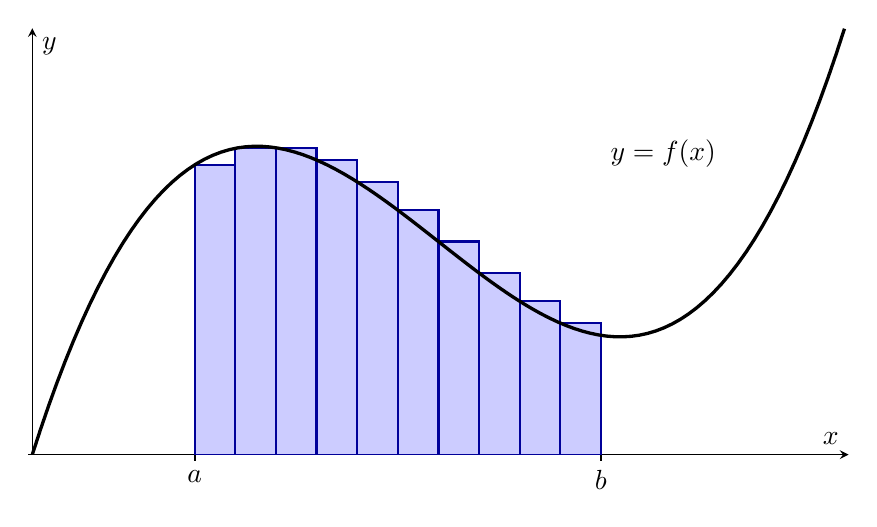
\begin{tikzpicture}
\begin{axis}[
    width=12cm,
    height=7cm,
    axis lines=middle,
    xlabel={$x$},
    ylabel={$y$},
    xmin=0, xmax=10,
    ymin=0, ymax=100,
    xtick={2, 7},
    xticklabels={$a$, $b$},
    ytick=\empty,
    samples=100,
    domain=0:10,
    enlargelimits={abs=0.05},
    tick style={black, thick},
    major tick length=0.15cm,
    xticklabel style={font=\normalsize},
]


% Draw Riemann sum rectangles (left endpoint)
\foreach \i in {0,...,9} {
    \pgfmathsetmacro{\xleft}{2 + \i*0.5}
    \pgfmathsetmacro{\xright}{\xleft + 0.5}
    \pgfmathsetmacro{\height}{-15*(\xleft-5) + (\xleft-5)^3 + 50}
    \addplot[fill=blue!20, draw=blue!60!black, thick] coordinates {
        (\xleft, 0) (\xleft, \height) (\xright, \height) (\xright, 0)
    } -- cycle;
}

% The curve
\addplot[black, very thick, domain=0:10] {-15*(x-5) + (x-5)^3 + 50};

% Label for the function
\node[above right, black] at (axis cs:7, 65) {$y = f(x)$};

\end{axis}
\end{tikzpicture}
\caption{Riemann sum approximation of an integral}
\label{fig:riemann_sum}
\end{figure}

This information about differentials allows us to view the one attached to every integral in way beyond just useful notation.
Putting the formalism and rigorous definitions of integrals aside, they are fancy sums.
The area under a graph can be approximated by rectangles, as is shown by the above figure.
As the width of the rectangles decrease, the sums \href{https://commons.wikimedia.org/wiki/File:Riemann_sum_(leftbox).gif}{get closer} to the actual area under the curve.
That is, the limit of this sum is an integral.

Instead of thinking about it in terms of limits, we can imagine summing an infinite number of rectangles with infinitesimal width.
The height of a rectangle at some value of $x$ can be given by $f(x)$, so if the integral sums over areas, the $dx$ is the infinitesimal width.
This is all very imprecise and non-technical language.
However, it is enough to give us an intuitive feel of what an integral is and what the differential that is always attached to it means.

There is more to the peculiar symbol, though, and integrals are probably not the first place one would have spotted them.
That would instead be with regard to derivatives.
Indeed, the notation $dy/dx$ -- also attributed to Leibniz -- is very commonly used to denote the derivative of $y$ with respect to $x$.
When it is first taught to students at school, the warning will be given that it does not represent a fraction.
It just looks like a fraction, and treating it like a fraction works out almost all the time.

The resemblance it has to a ratio between two quantities is no coincidence, as Leibniz intended it to be just that: a ratio of infinitesimals.
The symbols $dx$ and $dy$ were used to represent infinitely small changes in $x$ and $y$ respectively.
Whilst we have, for the most part, left these imprecise notions behind, they will prove to be somewhat useful in understanding these symbols.\footnote{At the end of the day, the symbols mean whatever we want as long as it is consistent with the rest of our maths. That is why I gave the easy way out at the beginning, saying that the differential symbol in the integral can just be considered a part of the notation. However, as is being demonstrated, we can go further.}

\section{Differential of a Function}

Firstly, consider the fact that the derivative has many different notations.
The derivative of a function $f$ at $x$ may be expressed as $f'(x)$.
It follows that
\begin{equation*}
    \frac{dy}{dx} = f'(x).
\end{equation*}
This is just equating two things that are defined to mean the exact same thing.
Now, although the left-hand side is not a fraction, what if we rewrote the equation as follows?
\begin{equation*}
    dy = f'(x) \diff x
\end{equation*}
The right-hand side now looks exactly like an integrand.
This looks promising, but we did say beforehand that $dy/dx$ is not a fraction.
So, are we allowed to do that?
No. The symbols $dx$ and $dy$ have not been given a meaning outside of when they appear in $dy/dx$, so it makes no sense to separate them.
However, when something does not have meaning, we can always attempt to give it one and see where that leads us.

First, let $\Delta x$ be some real number, just as $x$ is.
Then, we can call $df$ the differential of $f$, a function of $x$.
The differential itself is a function of both $x$ and $\Delta x$, is defined as
\begin{equation*}
    df(x, \Delta x) \coloneq f'(x) \Delta x.
\end{equation*}
What was the point of that?
We went from performing an algebraic manipulation in a situation where it does not make sense, to creating a perfectly fine definition.
Since we have made it clear that $df$ is a function of two variables, we can write $df(x, \Delta x)$ as $df(x)$ or even $df$ (we are not changing the meaning).
The differential of the function $f(x) = x$ is given by
\begin{equation*}
    dx = 1 \cdot \Delta x = \Delta x
\end{equation*}
for all values of $x$.
This means that, even though $dx$ is technically still a function of $x$, we can just write $dx = \Delta x$.
With this, and by letting $y = f(x)$, we can rewrite our equation as
\begin{equation*}
    dy = f'(x) \diff x.
\end{equation*}
This looks exactly like what we already had, but now we have reached it by valid means.
We see that the differential $dy$ is defined in terms of $x$ and $dx$, and the differential $dx$ is essentially just some real number.
If we desired, we could go further to obtain $dy/dx = f'(x)$, but this can lead to confusion.
By that equation, $f'(x)$ equals a ratio of differentials that have each been separately defined.
However, $f'(x)$ is can be expressed with Leibniz's notation as $dy/dx$ -- which is not a ratio.\footnote{We cannot redefine the derivative to be a ratio of our two differentials. Their definitions involve the derivative, so it would be circular. Instead, view it as evidence for the self-consistency of Leibniz's notation}
This is just something to note.

We have now obtained our third interpretation of the differential, a function of two real numbers $x$ and $\Delta x$.
This can be extended to higher-order differentials, as well as to the differentials of multivariable functions.
Its usefulness is in the fact that it represents the principal part of the change of a function.
To see what that exactly means, consider some function\footnote{Technically, $f$ is the function and $f(x)$ is the value of the function at $x$.} $y=f(x)$ between two points $x$ and $x + \Delta x$.
Let $x$ be fixed.
The change in $x$ values is $\Delta x$ and the change in $y$ values is $\Delta y \coloneq f(x + \Delta x) - f(x)$.

By the definition of the derivative, $\Delta y / \Delta x \to f'(x)$ as $\Delta x \to 0$.
This means that for small $\Delta x$, we have $\Delta y / \Delta x \approx f'(x)$.
If the difference (or error) is $\varepsilon$, then $\Delta y / \Delta x = f'(x) + \varepsilon$.
Rearranging gives us
\begin{align*}
    \Delta y &= (f'(x) + \varepsilon) \Delta x \\
    &= f'(x) \Delta x + \varepsilon \Delta x \\
    &= dy + \varepsilon \Delta x.
\end{align*}
The change in $y$ is equal to a linear function of $\Delta x$, $dy$, plus a (generally) nonlinear error term.
Thus, $dy$ is the linear (or principal) part of $\Delta y$.
As $\Delta x \to 0$, we require that $\varepsilon \Delta x / \Delta x = \varepsilon \to 0$, i.e. the error term shrinks to zero faster than $\Delta x$.
This means that $\Delta y \to d y$, and $\Delta y \approx dy$ for small $\Delta x$.
An equivalent way to view the differential is as the best linear approximation to a function at some point.

Let us look at one use case of this: approximating the values of functions.
What is the value of $\sqrt{90}$?
Since the function $y = \sqrt{x}$ is strictly increasing, we know that $\sqrt{90}$ will be between $\sqrt{81}=9$ and $\sqrt{100}=10$.
Let $x = 100$ and $\Delta x = -10$, so that $x + \Delta x = 90$.
Thus, $\Delta y = \sqrt{90} - \sqrt{100} = \sqrt{90} - 10$.
This means that $10 - \Delta y$ is the exact value of $\sqrt{90}$, but we do not know what $\Delta y$ is.
Our approximation from before comes in handy here.

The derivative of $\sqrt{x}$ is given by
\begin{equation*}
    f'(x) = \frac{1}{2\sqrt{x}}.
\end{equation*}
At $x=100$, we have $f'(x) = 1/20 = 0.05$.
This is all we need for our approximation.
\begin{align*}
    \sqrt{90} &= \Delta y + 10 \\
    &\approx dy + 10 \\
    &= f'(10) \Delta x + 10 \\
    &= 0.05 \cdot -10 + 10 \\
    &= 9.5
\end{align*}
The actual value of $\sqrt{90}$ is $9.47213595\ldots$, so we were just 0.62\% off.
The computations were incredibly easy, which is the case as long as we have nice values of the function and its derivative to work with.
We can illustrate the efficacy of this method with a diagram.

\begin{figure}[!htbp]
\centering
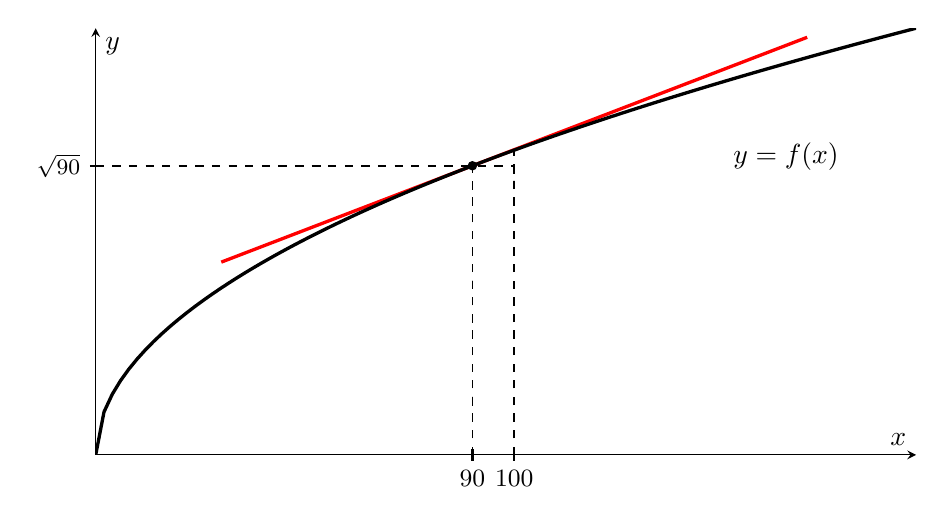
\begin{tikzpicture}
\begin{axis}[
    width=12cm,
    height=7cm,
    axis lines=middle,
    xlabel={$x$},
    ylabel={$y$},
    xmin=0, xmax=196,
    ymin=0, ymax=14,
    xtick={90, 100},
    xticklabels={90, 100},
    ytick={sqrt(90)},
    yticklabels={$\sqrt{90}$},
    samples=100,
    domain=0:196,
    enlargelimits=false,
    tick style={black, thick},
    major tick length=0.15cm,
    xticklabel style={font=\small},
]

\addplot[red, very thick, domain=30:170] {x/(2*sqrt(90)) + (sqrt(90) - 90/(2*sqrt(90)))};

% The curve
\addplot[black, very thick, domain=0:196] {sqrt(x)};

\draw[fill] (axis cs:{90,sqrt(90)}) circle [radius=1.5pt];
\addplot[black, semithick, dashed, domain=0:100] {sqrt(90)};
\addplot[black, semithick, dashed, domain=0:90] (90, {sqrt(x)});

\addplot[black, semithick, dashed, domain=0:100] (100, {sqrt(x)});

% Label for the function
\node[above right, black] at (axis cs:150, 9) {$y = f(x)$};

\end{axis}
\end{tikzpicture}
\caption{Linear approximation of $\sqrt{90}$}
\label{fig:linaer_approximation}
\end{figure}

We calculated $dy$, the increase in the tangent, as an approximation to $\Delta y$, the increase in the function.
As can be seen from the figure, these are very similar values.
Since $f'(x) \to 0$ as $x \to \infty$ (the curve flattens), this method of approximation gets better for larger square roots.
That does not mean that this method is not useful for other functions, as it is generally applicable to functions that are sufficiently `nice' -- where a discussion on `niceness' is beside the point.

Another example is approximating $\ln 3$.
We know that $\ln e$ is 1, and $e \approx 3$.
Let $x = e$ and $\Delta x = 3 - e$, so that $x + \Delta x = 3$.
Then, $\Delta y = \ln 3 - \ln e = \ln 3 - 1$.
The derivative of $\ln x$ is simply $1/x$, so we have
\begin{equation*}
    \ln 3 \approx \frac{1}{e} \cdot (3 - e) + 1 = \frac{3}{e}.
\end{equation*}
The number $e$ is well-known enough for us to use its value for the approximation, giving us $\ln 3 \approx 1.104$.
The actual value is $1.09861229\ldots$, which means that there is a 0.46\% error.
These approximations are known as linear approximations, and they have a fair bit of applications.
The idea of calculating the linear part of $\Delta y$ can be made more precise with \emph{Taylor's theorem}, though it is not necessary to understand the method itself.

\section{Reinterpreting Formulae}

Now that we have a formal definition of a differential, it would be useful to use what we have to look at commonly-known formulae in this new context.
First is the chain rule for derivatives.
Given two functions $f$ and $g$, the derivative of their composition $f \circ g$ is given by
\begin{equation*}
    f'(g(x)) g'(x).
\end{equation*}
If we write $y = f(g(x))$ and $u = g(x)$, then the previous fact can be rewritten as
\begin{equation*}
    \frac{dy}{dx} = \frac{dy}{du} \frac{du}{dx}
\end{equation*}
using Leibniz's notation.
The latter way is writing is more elegant both in this case, and for compositions of more than two functions.
It reinforces the idea of the derivative being a fraction, even though it is not.
If we were to, however, consider the terms on the RHS as being differentials, then we do have fractions -- which can cancel.
\begin{align*}
    \frac{dy}{du} \frac{du}{dx} = \frac{y'(x) \diff x}{u'(x) \diff x} \frac{u'(x) \diff x}{dx} = y'(x)
\end{align*}
Of course this is not a proof of the chain rule.
It does not show that the fraction $dy/du$ is the same as the derivative of $y$ with respect to $u$, and it does not work when $u'(x) = 0$ wherever we are differentiating at.
Regardless, it shows the chain rule to be intuitively very simple -- just `cancelling' fractions.

Our definition of differentials can also be shown to be insightful with regard to integration by substitution and the method of solving differential equations by separation of variables.
That would make sense, as they are both linked to the chain rule (with the former being an inverse to some degree).
Given two functions $f$ and $g$, the integration by substitution formula states that
\begin{equation*}
    \int_{a}^{b} f(g(x))g'(x) \diff x = \int_{g(a)}^{g(b)} f(u) \diff u.
\end{equation*}
By making the substitution $u = g(x)$, we know that the differential of $u$ is given by $du = g'(x) \diff x$.
This suggests that the formula above is a literal substitution of one variable with another.
The limits being transferred from $x=a$ and $x=b$ to $u=g(a)$ and $u=g(b)$ make sense as well.\footnote{We could have had the limits on the RHS integral be $x=a$ and $x=b$ if we really wanted. This shows that nothing `actually' changes between the two integrals.}
Without the integral symbols, the equation would just be something that follows directly from the definition of a differential.
If it were possible to integrate a differential in the sense of it being the whole integrand -- not just integrating a function -- then the formula would be completely trivial.

Now, on to the topic of differential equations.
Let $f$, $g$, and $h$ be functions that satisfy the differential equation
\begin{equation*}
    \frac{dy}{dx} = g(x)h(y),
\end{equation*}
with $y=f(x)$.
If we treat the $dy$ in $dy/dx$ as a differential (which is a bit awkward notationally but valid), then we have a fraction that can be separated.
Multiplying both sides by $dx$ and dividing by $h(y))$ gives
\begin{equation*}
    \frac{dy}{h(y)} = g(x) \diff x.
\end{equation*}
This is really the same as
\begin{equation*}
    \frac{f'(x)}{h(f(x))} \diff x = g(x) \diff x.
\end{equation*}
Since $dx$ is some real number, we can cancel it out and then integrate both sides with respect to $x$ in order to solve the equation.
However, our integrals will have $dx$ at the end anyway.
What was the point of cancelling them out beforehand?
The $dx$ in an integral is still different from the $dx$ we have defined to be equal to some real number $\Delta x$.
Once again, if we could just integrate the differentials directly, things would be much simpler.

\section{Generalizing Differentials}

As was suggested at the end of the previous section, there is a different way to handle differentials that works well with integration.
Before that, we will have to perform quite a bit of work to generalize the notion of a differential; our current definition only works for functions of the type $\R \to \R$.
We will first cover higher-order differentials, which correspond to higher-order derivatives.
This is technically not a `generalization' in that it requires no new definitions.
The second-order differential, or second differential, of a function is given by finding the differential of the differential.
\begin{equation*}
    d^2 y \coloneq d(dy) = d(f'(x)\diff x) = (df'(x)) \diff x = f''(x) (dx)^2
\end{equation*}
Dividing through by $(dx)^2$ gives an equation very similar to Leibniz's notation for higher-order derivatives.
However, note that it is not a definition (as it would be if we were considering it as just notation).
\begin{equation*}
    \frac{d^2 y}{(dx)^2} = f''(x)
\end{equation*}
This is an interesting detail, again showing the efficacy and practicality of the notation.
Repeated applications of the differential gives us the general formula for the $n$-th order differential of $f$.
\begin{equation*}
    d^n y = d^n f(x, dx) = f^{(n)}(x) (dx)^n,
\end{equation*}
where $f^{(n)}$ is the $n$-th derivative of $f$.
This is pretty simple, but it only works under the assumption that $dx$ is itself not a function of $x$.
This might not be the case.
An example where $dx$ depends on $x$ is if $x$ depends on some parameter $t$.
The first-order differential is still given by $df(x, \Delta x) = f'(x) \Delta x = f'(x)\diff x$.
Since $x$ depends on $t$, $\Delta x$ depends on $t$ as well.\footnote{This is not a logical consequence, but rather a sensible choice we make. We choose to define $\Delta x$ as an actual change $x(t+\Delta t) - x(t)$, now that we are able to, instead of it just being some real number which represents the concept of change only when put in context.}
The principal part of the change $\Delta x$ is given by $dx = x'(t) \diff t$.
The reasoning for this is not new, as we are simply applying our definition of the differential to $x$ now that it is a function of $t$.
Then, $df$ is given by
\begin{equation*}
    df = f'(x)x'(t) \diff t.
\end{equation*}
This is essentially just the chain rule applied to differentials.
Finding $d^2 f$ will involve differentiating with respect to $t$ instead of $x$ to avoid concerning ourselves with whether $dx$ can be expressed as a function of $x$.
For this, we need the product rule.
\begin{equation*}
    d^2 f = f''(x) (x'(t)\diff t)^2 + f'(x) x''(t) (dt)^2
\end{equation*}
Simplifying this using $dx = x'(t)\diff t$ and $d^2 x = x''(t) (dt)^2$ gives us
\begin{equation*}
    d^2 f = f''(x) (dx)^2 + f'(x) d^2 x.
\end{equation*}
Note that differentiating with respect to $x$ directly would still have given us the same answer (even if it might not be technically valid).
This result generalizes to third derivatives, fourth derivatives, and so on.
The general formula for the $n$-th order differential is not at all insightful, so it will not be provided.
Higher-order differentials in general are not particularly relevant to the rest of our discussion, but they have been included for completeness.

Now we will consider multivariable functions.
Let $f\colon \R^n \to \R$, so it maps $n$ real numbers to a single real number.
It can equivalently be considered a function of $n$ independent variables, and we may write $y = f(x_1, \ldots, x_n)$.
There are multiple sensible ways of defining the differential.
We will first cover the simpler of the two approaches, before we cover the second and show that they are actually the same thing.
The total change in $y$ is given by
\begin{equation*}
    \Delta y = \Delta f \coloneq f(x_1 + \Delta x_1, \ldots, x_n + \Delta x_n) - f(x_1, \ldots, x_n),
\end{equation*}
where $\Delta x_i$ is a real number.
We are able to split this change into a linear (principal) part and a nonlinear part (which we call the error).
Each $x_i$ will contribute to the total change, both in its principal part and error part.
The former is given by
\begin{equation*}
    \frac{\partial y}{\partial x_i} \Delta x_i,
\end{equation*}
which we will cause the partial differential of $y$ with respect to $x_i$.
The error is simply $\varepsilon_i \Delta x_i$.
This is a natural extension of the one-dimensional case, with the primary difference being that we have now many more terms.
We can find the total principal change in $y$ due to the changes in all the variables by summing the partial differentials.
The result of this sum will be called the total differential of $y$.
\begin{equation*}
    dy \coloneq \sum_{i=1}^{n} \frac{\partial y}{\partial x_i} \Delta x_i
\end{equation*}
Since $dx_i(\Delta x_1, \ldots, \Delta x_n) = \Delta x_i$ (the partial derivative equals one for this term and zero for all others), we can rewrite the differential as
\begin{equation*}
    dy = \sum_{i=1}^{n} \frac{\partial y}{\partial x_i} \diff x_i.
\end{equation*}
As all $\Delta x_i \to 0$, we have $\varepsilon_i \to 0$, so $dy \to \Delta y$.
Just as in the case of one variable, this is approximately equal to the actual change in $y$: $\Delta y \approx \diff y$ (for small changes in $x_i$).
Their use cases are also similar.
However, their increased generality makes them much more applicable to situations -- including estimating error in measurements.

Since our function $f$ takes a list of numbers, and a list of numbers can be represented by a vector, we can consider $f$ to map $n$-dimensional vectors to real numbers.
This will not change anything about the above formula; we are now just considering the components of $\mathbf{x}$ and $d\mathbf{x}$.
We can go a step further by consider functions that output vectors as well.
Let $\mathbf{f}\colon \R^n \to \R^m$, with $y = \mathbf{f}(\mathbf{x})$.
The only thing that changes is that we are now differentiating vectors, which we do by differentiating their components separately.
This gives us a slightly modified formula for the total differential.
It is just a change of notation.
\begin{equation*}
    d\mathbf{f}(\mathbf{x}) = \sum_{i=1}^{n} \frac{\partial\mathbf{f}}{\partial x_i} \diff x_i
\end{equation*}
When we generalize to vector-valued functions, the changes in our function are no longer a real number.
It thus makes sense that the differential is not a real number any more, either.
Functions that map vectors to vectors will be as general as we go for now.
Although, as we stated before, we will offer a different perspective on what we just derived.
Once again, consider $\mathbf{f}\colon \R^n \to \R^m$, with $\mathbf{x}$ and $\Delta\mathbf{x}$ being in $\R^n$.
The total change in $\mathbf{f}$ is given by
\begin{equation*}
    \Delta \mathbf{f} = \mathbf{f}(\mathbf{x} + \Delta\mathbf{x}) - \mathbf{f}(\mathbf{x}).
\end{equation*}
This is a rewritten version of what we had before.
We want this total change to be equal to a linear change, as well as an error term.
Note that we had $\Delta f = df + \varepsilon\Delta x$ in the one-dimensional case, with $df = f'(x) \diff x$.
Our multivariable version of the derivative is the Jacobian matrix, $\mathbf{J_f}$.
The linear change is then $\mathbf{J_f}(\mathbf{x})\Delta\mathbf{x}$.
The error term is given by\footnote{It is not $\norm{\boldsymbol{\varepsilon}}\Delta\mathbf{x}$ instead because that would give an $n$-dimensional vector whilst the other terms are $m$-dimensional.} $\norm{\Delta\mathbf{x}}\boldsymbol{\varepsilon}$, with $\boldsymbol{\varepsilon} \to \mathbf{0}$ as $\Delta\mathbf{x} \to \mathbf{0}$.
We thus know that the total change in $\mathbf{f}$ can be expressed as follows.
\begin{equation*}
    \Delta\mathbf{f} = \mathbf{J_f}(\mathbf{x})\Delta\mathbf{x} + \norm{\Delta\mathbf{x}}\boldsymbol{\varepsilon}
\end{equation*}
The differential of $\mathbf{f}$ is given by
\begin{equation*}
    d\mathbf{f}(\mathbf{x}, \Delta\mathbf{x}) = \mathbf{J_f}(\mathbf{x})\Delta\mathbf{x}.
\end{equation*}
For $\mathbf{f}(\mathbf{x}) = \mathbf{x}$, it can be shown that for all $\mathbf{x} \in \R^n$, the Jacobian $\mathbf{J_f}(\mathbf{x}) = \mathbf{I}$, the identity matrix.
This means that $d\mathbf{x} = \mathbf{I}\Delta\mathbf{x} = \Delta\mathbf{x}$ for all $\mathbf{x}$.
We can therefore rewrite the differential of $\mathbf{f}$ as
\begin{equation*}
    d\mathbf{f}(\mathbf{x}) = \mathbf{J_f}(\mathbf{x}) \diff\mathbf{x}.
\end{equation*}
This differential is exactly the same as the total differential we previously derived.
To show this, we simply perform the matrix multiplication.
\begin{equation*}
    \mathbf{J_f}(\mathbf{x}) \diff\mathbf{x} = \begin{bmatrix}
        \dfrac{\partial f_1}{\partial x_1} & \cdots & \dfrac{\partial f_1}{\partial x_n} \\[0.5em]
        \vdots & \ddots & \vdots \\[0.5em]
        \dfrac{\partial f_m}{\partial x_1} & \cdots & \dfrac{\partial f_m}{\partial x_n}
    \end{bmatrix}
    \begin{bmatrix}
        dx_1 \vphantom{\dfrac{\partial f_1}{\partial x_n}}\\[0.5em]
        \vdots \\[0.5em]
        dx_n \vphantom{\dfrac{\partial f_m}{\partial x_n}}
    \end{bmatrix}
    = \begin{bmatrix}
        \dfrac{\partial f_1}{\partial x_1}\diff x_1 + \cdots + \dfrac{\partial f_1}{\partial x_n}\diff x_n\\[0.5em]
        \vdots \\[0.5em]
        \dfrac{\partial f_m}{\partial x_1}\diff x_1 + \cdots + \dfrac{\partial f_m}{\partial x_n}\diff x_n
    \end{bmatrix}
    = \sum_{i=1}^{n} \frac{\partial\mathbf{f}}{\partial x_i} \diff x_i
\end{equation*}
Whilst the two results are equivalent, the form involving the Jacobian is usually preferred.
It is much more compact and clear (as long as the definition and notation is understood).
The Jacobian better represents the nature of a derivative of as a linear map and not necessarily a number.
As a bonus, $d\mathbf{f}(\mathbf{x}) = \mathbf{J_f}(\mathbf{x})\diff\mathbf{x}$ maintains a similar form to the one-dimensional version of the differential.
The other form may be better-suited for quick computations, however.

We have now obtained an interpretation of the differential for a more general class of functions. 
It is a function of $\mathbf{x}$ and $d\mathbf{x}$, representing the principal change in the function.
This generalization, and the work done to formalize the derivative of functions of type $\R^m \to \R^n$, falls under the concept of the \href{https://en.wikipedia.org/wiki/Fr%C3%A9chet_derivative}{Fre\'chet derivative}.
This derivative can be defined on even more general spaces, but that is beyond the scope of our discussion.

A useful concept that is related to -- but distinct from -- our definition of the differential is the directional derivative.
\begin{equation*}
    \nabla_\mathbf{v}\mathbf{f}(\mathbf{x}) \coloneq \lim_{t \to 0} \frac{\mathbf{f}(\mathbf{x}+t\mathbf{v}) - \mathbf{f}(\mathbf{x})}{t}
\end{equation*}
Here, $\nabla_\mathbf{v}\mathbf{f}$ is the directional derivative of $\mathbf{f}$ along some vector $\mathbf{v}$.
This is a weaker concept of the derivative than what we were previously using.
If function $\mathbf{f}$ is differentiable at a point $\mathbf{x}$ (the Jacobian exists), then all directional derivatives at that point will exist.
The converse of this statement is not true.
The relationship between the directional derivative and the Jacobian is that $\mathbf{J_f}(\mathbf{x})\mathbf{v} = \nabla_\mathbf{v}\mathbf{f}(\mathbf{x})$, meaning that $d\mathbf{f}(\mathbf{x}, \mathbf{v}) = \nabla_\mathbf{v}\mathbf{f}(\mathbf{x})$.
The directional derivative can be thus be written as
\begin{equation*}
    \nabla_\mathbf{v} \mathbf{f}(\mathbf{x}) = \sum_{i=1}^{n} \frac{\partial\mathbf{f}}{\partial x_i} v_i,
\end{equation*}
where $\mathbf{v} = \langle v_1, v_2, \ldots, v_n \rangle$.
The map $\eval*{\nabla_\mathbf{v}}{\mathbf{x}}$ can similarly be written as a sum of maps.
\begin{equation*}
    \eval{\nabla_\mathbf{v}}{\mathbf{x}} = \sum_{i=1}^{n} v_i \eval{\frac{\partial}{\partial x_i}}{\mathbf{x}}
\end{equation*}
This will be useful later.

\section{Tangent Spaces}

Whilst our notation for the differential is standard when concerning functions defined on Euclidean space ($\R^n$), it will overlap with the notation for new concepts that we will introduce.
We will use $D\mathbf{f}$ instead of $d\mathbf{f}$ to denote the differential of function.
This also replaces $d\mathbf{x}$ with $D\mathbf{x}$, but we will instead keep to using $\Delta\mathbf{x}$; even this will be replaced later.
Unfortunately, there is no better way to handle the many different notations available whilst always attempting to use relatively standard ones for each topic.

In order to move on to the next step of developing a `differential' that works well with integration, we will have to shift our perspective and create new definitions.
Previously, we have been considering $D\mathbf{f}$ as a function of two numbers, $\mathbf{x}$ and $\Delta\mathbf{x}$.
Another way to view it is by fixing the variable $\mathbf{x}$ to consider the differential at a specific point.
We then have $D\mathbf{f_x}$ as a function of just $\Delta\mathbf{x}$.
Currently, $\Delta\mathbf{x}$ just represents some number which can be thought of as the change between $\mathbf{x}$ and some other point.
In practice, we want it to be small change.
The smaller it is, the close the principal change $D\mathbf{f}$ is to the total change $\Delta\mathbf{f}$.

Although the following language is not precise, we can say that these changes would be equal if $\Delta\mathbf{x}$ was infinitely small.
A point established near the start of this exposition was that the concept of infinitesimals is dated.
However, instead of abandoning them completely, we will show one way in which they can be formalized.
Whilst the concept of an infinitesimal itself is vague (as is), it is closely related to tangents.
Regardless of whether a derivative is interpreted as the ratio of infinitesimals, or as a limit, it can be thought of as the gradient of a tangent line.

Quantities that are the derivative of other quantities are always tangents.
For example, the instantaneous velocity vector $\mathbf{v} = \mathbf{\dot{r}}$ of a particle with position vector $\mathbf{r}$ is tangent to the trajectory of the particle.
The trajectory or path of the particle is the space of all points that $\mathbf{r}$ lands on.
With this information, we make the choice to reinterpret an infinitesimal change as a tangent vector.
Instead of being a change at all, $\Delta\mathbf{x}$ can be considered a vector tangent to $\R^n$ at the point $\mathbf{x}$.
The differential $D\mathbf{f_x}$ can now be considered a function of tangent vectors.

The set of all the tangent vectors of $\R^n$ at $\mathbf{x}$, the domain of $D\mathbf{f_x}$, forms a vector space.
This vector space is called the \emph{tangent space} of $\R^n$ at $\mathbf{x}$, denoted by $T_\mathbf{x}\R^n$.
What actually are the tangent vectors here?
To see that, it would be helpful to simplify to the plane $\R^2$ first.
Here, $T_\mathbf{x} \R^2$ is the collection of vectors starting at $\mathbf{x}$ tangent to $\R^2$; they all lie flat on the plane.
This seems almost identical to $\R^2$ itself, except for the origin of the vectors.
Indeed, there is a natural way to associate $\R^2$ and $T_\mathbf{x} \R^2$, so the spaces can be considered essentially the same.

The tangent spaces of $\R^2$ can be thought of as a copy of $\R^2$ attached to a particular point.
This generalizes to $\R^n$.
Now, we have found a way to describe the domain of the differential.
What about the codomain?
In all cases, $D\mathbf{f_x}$ represents a (very small) change in $\mathbf{f}(\mathbf{x})$.
Using the same reasoning as before, an infinitesimal change can be formalized be considering $D\mathbf{f_x}$ to be a tangent vector.
Thus, the codomain is the tangent space of $\R^m$ at the point $\mathbf{f}(\mathbf{x})$: $T_{\mathbf{f}(\mathbf{x})}\R^m$.
Putting this together, we have the differential $D\mathbf{f_x} \colon T_\mathbf{x}\R^n \to T_{\mathbf{f}(\mathbf{x})}\R^m$ defined by $D\mathbf{f_x}(\Delta\mathbf{x}) = \mathbf{J_f} \Delta \mathbf{x}$.

It would seem that the notion of a tangent space is not particularly useful, since $T_\mathbf{x} \R^n$ is practically the same as $\R^n$.
This is the case if we look at nothing but Euclidean spaces.
What other spaces can we look at?
For this, we will introduce the concept of a \emph{manifold}.
A manifold is a space where the idea of closeness between points exists, but not necessarily the ability to measure distances and angles.\footnote{The technical term for this is that a manifold is a topological space.}
Additionally, a manifold resembles Euclidean space near each point.
This is a very informal definition of a manifold, though it is all we need for this exposition.

Examples of a one-dimensional manifold include line segments, the real line $\R$, circles.
It can also be a collection of these, since a manifold can have multiple disconnected pieces.
Requiring a manifold to resemble a single Euclidean space $\R^n$ at every point, which is in the usual definition, means that these pieces must have the same dimension. 
Examples of two-dimensional manifolds include spheres, the plane $\R^2$, and a torus (doughnut).
In general, most shapes and spaces that one would imagine which do not cross themselves are examples of manifolds.

An example of a space that is not a manifold is an infinity symbol, due to the curve crossing with itself at the centre.
If we remove the central point, then the neighbourhood around it looks like four connected parts.
If we remove a point from the real line, then its neighbourhood looks like two connected parts.
Thus, the shape does not resemble Euclidean space near every point.
Other examples are two cones combines to make an hourglass shape, and more exotic shapes such as many fractals.
All it takes is for at least one point to not locally resemble Euclidean space.

Another important aspect of manifolds is the distinction between the manifold itself and the ambient space that a manifold may be embedded in.
For instance, a circle may be embedded in $\R^2$, or $\R^3$, or even inside a sphere.
When visualizing manifolds, we always use some embedding, e.g. a circle is drawn in a plane.
Properties of manifolds, such as its tangent spaces, these are intrinsic to the manifold itself; they do not depend on what the manifold is embedded in, if there is any embedding at all.
In general, we will talk about manifolds by themselves and their intrinsic properties, as opposed to extrinsic properties.

Whenever we mention manifolds, we will actually be referencing smooth manifolds in particular.
They are `smooth' in the way one would usually think of, so regular manifolds such as triangles, squares, and cones are excluded due to their sharp corners.
However, it more importantly means that we are able to do perform calculus with them.
This additional structure is required for everything we wish to do with manifolds, including tangent spaces.
Additional structure can be added to a manifold to allow for distances and angles to be measured, though our manifolds will only have this if specified.
We will also usually consider smooth (infinitely differentiable) functions on these manifolds.

The final disclaimer to make is that our manifolds will be orientable manifolds.
For instance, a circle might have a clockwise or anticlockwise orientation.
We will require this for actually integrating over the manifolds, which is why we have introduced them in the first placed.
Whilst integration on nonorientable manifolds can be defined, but it is beside the point of what we wish to show with this exposition.
All of these caveats should be expected considering how general of an idea that we have introduced.
The advantage is that our theory of integration will be considerably more powerful than what we had to work with before.

We may now talk about tangent spaces that are actually interesting.
Let us consider the unit circle, which is denoted by $\mathbb{S}^1$.
The tangent space of $\mathbb{S}^1$ at some point $p$, $T_p \mathbb{S}^1$, is the line tangent to the circle at $p$.
This can be seen in \cref{fig:circle_tangent}.

\begin{figure}[!htbp]
\centering
\begin{tikzpicture}[scale=1.4]
    % Draw the unit circle
    \draw[black, thick] (0,0) circle (2cm);
    
    % Mark the point in the first quadrant (at 45 degrees)
    \pgfmathsetmacro{\angle}{45}
    \pgfmathsetmacro{\px}{2*cos(\angle)}
    \pgfmathsetmacro{\py}{2*sin(\angle)}
    
    % Draw the tangent line
    \draw[red, thick] ({\px - 1.5*sin(\angle)}, {\py + 1.5*cos(\angle)}) -- 
                       ({\px + 1.5*sin(\angle)}, {\py - 1.5*cos(\angle)});
    
    % Draw the point
    \filldraw (\px,\py) circle (2pt) node[above right] {$p$};
    
    % Draw axes
    \draw[-latex] (-2.5,0) -- (2.5,0) node[right] {$x$};
    \draw[-latex] (0,-2.5) -- (0,2.5) node[above] {$y$};
\end{tikzpicture}
\caption{Tangent space of $\mathbb{S}^1$ at point $p$}
\label{fig:circle_tangent}
\end{figure}

Similarly, the tangent space of a sphere at $p$, $T_p\mathbb{S}^2$ is the plane tangent to the sphere at $p$.
This is shown in \cref{fig:sphere_tangent}.
An interesting thing to note, and the reason why a circle is $\mathbb{S}^1$ and a sphere is $\mathbb{S}^2$, is that the dimension of these manifolds are one and two, respectively.
A circle resembles a line near a point, and a sphere resembles a plane near a point.
On the other hand, a disk is two-dimensional and ball is three-dimensional.
Note that their boundaries are the circle and sphere, which have one fewer dimension than them.
This relationship between the dimension of a manifold and its boundary is true in general.

When people first learn about shapes, they learn that a circle is two-dimensional and a sphere is three-dimensional.
This is in reference to the smallest Euclidean space the shape can be embedded in; one cannot embed a circle into a line.
Under this definition, the dimension of the disk and ball are still the same.
This is an extrinsic definition.
Both interpretations are correct \cite{shape_dimension_convention} depending on the convention we have for what the dimension of a shape is.
We use the intrinsic dimension.

\begin{figure}[!htbp]
\centering
\tdplotsetmaincoords{70}{110}

\begin{tikzpicture}[scale=1.2]
    %--- 2D shaded "sphere" (visual only) ---
    \def\R{2.5} % sphere radius
    \shade[ball color=white!90!blue, opacity=0.85] (0,0) circle (\R);

    %--- 3D drawing using tikz-3dplot ---
    \begin{scope}[tdplot_main_coords]

        % coordinates of point p on sphere: p = R * (1,1,1)/sqrt(3)
        \pgfmathsetmacro{\pval}{\R/sqrt(3)}
        \coordinate (O) at (0,0,0);
        \coordinate (P) at (\pval,\pval,\pval);

        % Build an orthonormal tangent basis at P:
        % u = (1,-1,0)/sqrt(2)
        \pgfmathsetmacro{\ux}{1/sqrt(2)}
        \pgfmathsetmacro{\uy}{-1/sqrt(2)}
        \pgfmathsetmacro{\uz}{0}

        % n = (1,1,1)/sqrt(3)  (unit normal)
        \pgfmathsetmacro{\nx}{1/sqrt(3)}
        \pgfmathsetmacro{\ny}{1/sqrt(3)}
        \pgfmathsetmacro{\nz}{1/sqrt(3)}

        % v = n x u  (already unit length because n and u are unit & orthogonal)
        \pgfmathsetmacro{\vx}{\ny*\uz - \nz*\uy} % = 1/sqrt(6)
        \pgfmathsetmacro{\vy}{\nz*\ux - \nx*\uz} % = 1/sqrt(6)
        \pgfmathsetmacro{\vz}{\nx*\uy - \ny*\ux} % = -2/sqrt(6)

        % plane half-size (controls how large the drawn patch is)
        \pgfmathsetmacro{\psize}{1.6}

        % compute plane corners: P + s*(±u ± v)
        \pgfmathsetmacro{\Ax}{\pval + \psize*(-\ux - \vx)}
        \pgfmathsetmacro{\Ay}{\pval + \psize*(-\uy - \vy)}
        \pgfmathsetmacro{\Az}{\pval + \psize*(-\uz - \vz)}
        \coordinate (A) at (\Ax,\Ay,\Az);

        \pgfmathsetmacro{\Bx}{\pval + \psize*( \ux - \vx)}
        \pgfmathsetmacro{\By}{\pval + \psize*( \uy - \vy)}
        \pgfmathsetmacro{\Bz}{\pval + \psize*( \uz - \vz)}
        \coordinate (B) at (\Bx,\By,\Bz);

        \pgfmathsetmacro{\Cx}{\pval + \psize*( \ux + \vx)}
        \pgfmathsetmacro{\Cy}{\pval + \psize*( \uy + \vy)}
        \pgfmathsetmacro{\Cz}{\pval + \psize*( \uz + \vz)}
        \coordinate (C) at (\Cx,\Cy,\Cz);

        \pgfmathsetmacro{\Dx}{\pval + \psize*(-\ux + \vx)}
        \pgfmathsetmacro{\Dy}{\pval + \psize*(-\uy + \vy)}
        \pgfmathsetmacro{\Dz}{\pval + \psize*(-\uz + \vz)}
        \coordinate (D) at (\Dx,\Dy,\Dz);

        % draw the tangent plane patch
        \filldraw[fill=red!20,opacity=0.6,draw=red!60] (A) -- (B) -- (C) -- (D) -- cycle;

        % optional: draw the plane edges a bit thicker and semi-transparent
        \draw[red!60,very thick,opacity=0.6] (A) -- (B) -- (C) -- (D) -- cycle;

        % draw the great circle (equator in z=0 plane)
        % Front half (solid) - top half, y > 0
        \draw[thick,domain=-75:100,samples=40,variable=\t]
            plot ({\R*cos(\t)},{\R*sin(\t)},0);
        % Back half (dashed) - bottom half, y < 0
        \draw[dashed,thick,domain=90:290,samples=40,variable=\t]
            plot ({\R*cos(\t)},{\R*sin(\t)},0);

        % 3D axes
        \draw[-latex] (0,0,0) -- (7,0,0) node[right] {$x$};
        \draw[-latex] (0,0,0) -- (0,3.5,0) node[above] {$y$};
        \draw[-latex] (0,0,0) -- (0,0,3.5) node[above] {$z$};

        % mark P
        \filldraw (P) circle (1.8pt) node[above right=2pt] {$p$};

    \end{scope}

    % outer sphere outline in 2D (to sit on top of the shading)
    \draw[thick] (0,0) circle (\R);

\end{tikzpicture}
\caption{Tangent space of $\mathbb{S}^2$ at point $p$}
\label{fig:sphere_tangent}
\end{figure}

With these examples, we can see that a tangent space is generally distinct from underlying manifold in a meaningful way.
Now, it only makes sense to generalize to functions $f \colon M \to N$, where $M$ and $N$ are manifolds.
The more common name for the differential $Df_p \colon T_p M \to T_{f(p)} N$ in this context is the \emph{pushforward}.
It pushes tangent vectors on $M$ forward to tangent vectors on $N$.
This is a point where we can stop generalizing.
Although we have focused on Euclidean spaces, the idea of the pushforward is applicable to manifolds in general without needing to stray from our initial intuition.

Before we go on further, we will make some more changes to our notation.
Normally, the components of a vector $\mathbf{v}$ are denoted by $v_i$, with the index always on the bottom right.
We will now denote vector components with their index on the top right, e.g. $v^i$.
For basis vectors, the index is still on the bottom right, e.g. $\mathbf{\hat{e}}_i$.
The reason for this relates to how the components change under coordinate transformations (\emph{covariance} and \emph{contravariance}).
However, this is not important for our discussion, so it can simply be taken as a fact that this is something we do.

Another minor change to our notation will be that we will now only use boldface letters for vectors that are explicitly denoted to be Euclidean.
This means that tangent vectors will be written just like regular variables, also meaning that we will now use $f$ instead of $\mathbf{f}$ when concerned with functions of tangent vectors.
This is the case for manifolds in general, though they are not necessarily vector spaces in the first place.
All of this is to align ourselves with the standard conventions that exist concerning the topics we are discussing.

We now wish to provide a formal definition for a tangent space.
If our manifold is $\R^n$, this is easy to do.
A perfectly valid definition of $T_\mathbf{x} \R^n$ is the set $\mathbf{x} \times \R^n = \{(\mathbf{x}, \mathbf{v}) : \mathbf{v} \in \R^n\}$, so a tangent vector is a pair $(\mathbf{x}, \mathbf{v})$.
Attempting to generalize this to manifolds in general runs into the problem we just mentioned.
For example, the tangent space of the unit circle $\mathbb{S}^1$ at a point $p$ can be considered to be the set $\{(p, \mathbf{v}) : \mathbf{v} \cdot \mathbf{\hat{r}} = 0, \mathbf{v} \in \R^2\}$, where $\mathbf{\hat{r}}$ is the radial unit vector that points to $p$.
The ordered pair $(p, \mathbf{v})$ can indeed be thought of as an arrow starting at the point $p$ which is tangent to the circle, since $\mathbf{v}$ is orthogonal to the radius.

However, an arbitrary manifold does not have an inner product to work with.
This means that our approach will not work in general if the manifold is not embedded in Euclidean space.
This also relates to our previous visualizations of the tangent spaces for a circle and a sphere.
Thinking about tangent vectors as actual arrows tangent to a manifold will not work, because there is not an underlying space for them to point out into.
We mentioned earlier that tangent spaces are intrinsic, so there should be a way of describing them without an embedding.

It follows that a formal, intrinsic definition of a tangent space will be more abstract than we may have initially thought.
This does not mean that we will not be able to have any intuition for it.
In fact, we already have the intuition.
Using the definition we have, which Lee calls a ``geometric tangent space'' in his \textit{Smooth Manifolds} \cite[pp. 52--53]{Lee2012}, a tangent vector $(\mathbf{x}, \mathbf{v}) \in T_\mathbf{x} \R^n$ can be associated with the directional derivative map $\eval*{\nabla_\mathbf{v}}{\mathbf{x}}$.
As we know, it maps functions to real numbers.
Additionally, it satisfies the following properties, with $f, g \in C^\infty(\R^n)$ being smooth functions on $\R^n$ and $\lambda, \mu \in \R$.
\begin{itemize}
    \item $\eval{\nabla_\mathbf{v}}{\mathbf{x}}(\lambda f + \mu g) = \lambda\eval{\nabla_\mathbf{v}}{\mathbf{x}} f + \mu\eval{\nabla_\mathbf{v}}{\mathbf{x}} g$
    \item $\eval{\nabla_\mathbf{v}}{\mathbf{x}} fg = g(\mathbf{x})\eval{\nabla_\mathbf{v}}{\mathbf{x}}g + f(\mathbf{x})\eval{\nabla_\mathbf{v}}{\mathbf{x}}f$
\end{itemize}
That is, the map is linear, and it satisfies a condition very similar to the product rule for derivatives, which we call the \emph{Leibniz identity}.
Any map that satisfies these two properties is called a \emph{derivation}, and it can be seen as generalizing the concept of a derivative by possessing two of its important properties.
A derivation $v$ satisfies,
\begin{equation*}
    v(\lambda f + \mu g) = \lambda v(f) + \mu v(g),
\end{equation*}
and
\begin{equation*}
    v(fg) = v(f)g + fv(g).
\end{equation*}
It turns out to be the case that there is a one-to-one association between the space of all derivations at $\mathbf{x}$, linear maps $v \colon C^\infty (\R^n) \to \R$ that satisfy the Leibniz identity, and our ``geometric tangent space''.
This association is via the map from $(\mathbf{v}, \mathbf{x})$ to $\eval*{\nabla_\mathbf{v}}{\mathbf{x}}$.

We have shown that the space of derivations and our old tangent space are essentially the same in a way.
We are also able to easily define derivations on arbitrary manifolds $M$.
Thus, it is reasonable to define the tangent space of $M$ at a point $p \in M$, denoted $T_p M$, as the space of all derivations $v \colon C^\infty (M) \to \R$.
This includes $T_p \R^n$, replacing the ``geometric tangent space'' definition.
Now, it is still perfectly valid to think about tangent vectors as literal tangents to a manifold intuitively.
Abstracting the formal definition has not lost this intuition, which can be very helpful when thinking about these topics.

This allows us to give a proper definition of the pushforward $D\varphi_p \colon T_p M \to T_{\varphi(p)} N$ of a smooth function $\varphi \colon M \to N$, which were unable to do before.
We simply need a definition that maps derivations to derivations and simplifies to the old definition when we are dealing with Euclidean space.
Let $v \in T_p M$ be a tangent vector.
We define $D\varphi_p(v)$ to act on a smooth function $f \in C^\infty (N)$ as follows.
\begin{equation*}
    D\varphi_p(v)(f) \coloneq v(f \circ \varphi)
\end{equation*}
This is linear by the linearity of $v$.
Furthermore, it satisfies the Leibniz identity.
For any two smooth functions $f, g \in C^\infty (N)$, we have the following.
\begin{align*}
    D\varphi_p(v)(fg) &= v((fg) \circ \varphi) \\
    &= v((f \circ \varphi)(g \circ \varphi)) \\
    &= f \circ \varphi(p)v(g \circ \varphi) + g \circ \varphi(p)v(f \circ \varphi) \\
    &= f(\varphi(p)) D\varphi_p(v)(g) + g(\varphi(p)) D\varphi_p(v)(f)
\end{align*}
Hence, $D\varphi_p(v) \in T_{\varphi(p)} N$ is a derivation, so our definition is valid.
In the case where $M = \R^n$ and $N = \R^m$ (the letters are unfortunately mismatched), consider $v = \eval*{\nabla_\mathbf{v}}{p}$ with the associated Euclidean vector $\mathbf{v} \in \R^n$
We will make use of the expression of the directional derivative a sum using the standard basis for $\R^n$.
Let $x^1, x^2, \ldots, x^n$ represent the coordinates of $\R^n$, and let $y^1, y^2, \ldots, y^m$ represent the coordinates of $\R^m$.
We can apply the multivariable chain rule to $f \circ \varphi$.
This gives us
\begin{align*}
    D\varphi_p(v)(f) &= \eval{\nabla_\mathbf{v}}{p} (f \circ \varphi) \\
    &= \sum_{i=1}^{n}v^i \eval{\frac{\partial(f \circ \varphi)}{\partial x^i}}{p} \\
    &= \sum_{i=1}^{n} v^i \left(\sum_{j=1}^{m} \eval{\frac{\partial\varphi^j}{\partial x^i}}{p} \eval{\frac{\partial f}{\partial y^j}}{\varphi(p)}\right) \\
    &= \sum_{j=1}^{m} \left(\sum_{i=1}^{n} v^i \eval{\frac{\partial\varphi^j}{\partial x^i}}{p} \right) \eval{\frac{\partial f}{\partial y^j}}{\varphi(p)} \\
    &= \sum_{j=1}^{m} \eval{\nabla_\mathbf{v}}{p} (\varphi^j)\eval{\frac{\partial f}{\partial y^j}}{\varphi(p)}.
\end{align*}
Now, by letting $D\varphi_p (v) = w \in T_{\varphi(p)} \R^m$, we can identify the derivation $w$ with the associated Euclidean vector $\mathbf{w} \in \R^m$ via the directional derivative along $\mathbf{w}$.
This acts on $f$ to give
\begin{equation*}
    w(f) = \eval{\nabla_{\mathbf{w}}}{\varphi(p)} (f) = \sum_{j=1}^{m} w^j \eval{\frac{\partial f}{\partial y^j}}{\varphi(p)}.
\end{equation*}
Comparing this with the result we got above, we can see that
\begin{equation*}
    w^j = \eval{\nabla_\mathbf{v}}{p} (\varphi^j) = \nabla_\mathbf{v}\varphi^j(p),
\end{equation*}
Therefore,
\begin{equation*}
    \mathbf{w} = \nabla_\mathbf{v} \varphi(p) = \mathbf{J}_\varphi(p) \mathbf{v}.
\end{equation*}
Whilst it is technically incorrect to write $D\varphi_p(v) = \mathbf{J}_\varphi(p) \mathbf{v}$, they are essentially the same thing by the one-to-one association we have between tangent vectors (of a Euclidean space) and Euclidean vectors.
The pushforward for manifolds in general maintains the same interpretation as the old differential, representing the principal change in $\varphi$ or equivalently the best linear approximation to $\varphi$ at $p$.

Notice that our definition of the pushforward is completely independent of coordinates.
The fact that we can do this makes sense, as it captures geometric information about the manifold.
In general, we value coordinate-independent results for being more insightful as well as for the fact that we can apply them to any suitable coordinate system.
However, we need some coordinate system in order to preform calculations.
A basis for the tangent space $T_p \R^n$ can easily be created.
We know that each tangent vector can be represented by a directional derivative, and a directional derivative is a linear combination of partial derivatives.
For $v \in T_p \R^n$, we have
\begin{equation*}
    v = \eval{\nabla_\mathbf{v}}{p} = \sum_{i=1}^{n} v^i \eval{\frac{\partial}{\partial x_i}}{p} = \sum_{i=1}^{n} v^i \eval{\partial_{i}}{p},
\end{equation*}
for the associated $\mathbf{v} \in \R^n$; here, $\eval*{\partial/\partial x_i}{p}$ and $\eval*{\partial_{i}}{p}$ are just different notations.
It follows that $\{\eval*{\partial_1}{p}, \eval*{\partial_2}{p}, \ldots, \eval*{\partial_n}{p}\}$ is the standard basis for $T_p\R^n$.
The partial derivative $\eval*{\partial/\partial x_i}{p}$ is just a directional derivative along the Euclidean basis vector $\ehat_i$.
We now need a basis for the tangent space of an arbitrary smooth manifold $M$.
For this, we need coordinates for $M$.
The problem is that there is not necessarily one set of coordinates that can be used for the entirety of $M$.
There is generally not a sense of independent directions on a manifold, so we instead consider a coordinate system local to a point $p$, where $M$ resembles $\R^n$.

Given that $M$ has $n$ dimensions, our local coordinates $x^1, x^2, \ldots, x^n$ near $p$ are smooth functions from an (open) set $U \subseteq M$ to $\R$.
Although we have defined tangent vectors in relation to functions that are smooth on the entirety of $M$, we can identify a tangent vector in $T_p M$ with one in $T_p U$ without making any arbitrary choices.
The set $U$ can be arbitrarily small.
Thus, a tangent vector is a local object; if two smooth functions $f$ and $g$ are equal in a neighbourhood around $p$, then $v(f) = v(g)$.
It reasonably follows that a tangent vector $v \in T_p M$ is entirely determined by its action on the local coordinates.

Now, consider $n$ derivations $b_1, b_2, \ldots, b_n$ in $T_p M$.
We want these to be our basis tangent vectors, so we would want them to pick out the coordinates from a point.
\begin{equation*}
    b_i (x^j) = \begin{cases}
        1 & \text{if } i = j \\
        0 & \text{if } i \neq j
    \end{cases}
\end{equation*}
This is exactly how partial derivatives act.
\begin{equation*}
    \frac{\partial}{\partial x^i} x^j = \begin{cases}
        1 & \text{if } i = j \\
        0 & \text{if } i \neq j
    \end{cases}
\end{equation*}
Hence, just as we were able to use partial derivative operators to form the basis of $T_p \R^n$, we can use them for any smooth manifold $M$.
A basis of $T_p M$ is $\{\eval*{\partial_1}{p}, \eval*{\partial_2}{p}, \ldots, \eval*{\partial_n}{p}\}$.
Any tangent vector $v \in T_p M$ is can be expressed as a linear combination of these basis tangent vectors, and its $i$-th component is $v^i = v(x^i)$.
\begin{equation*}
    v = \sum_{i=1}^{n} v^i \eval{\partial_i}{p}
\end{equation*}
Often, we omit the evaluation at $p$ in the notation when it is unambiguous.
This is just to have nicer looking expressions.
The $i$-th component of $v$ can be obtained from its action on the local coordinate $x^i$.
This makes sense from what we know about tangent vectors, and it is shown below.
\begin{equation*}
    v(x^i) = \sum_{j=1}^{n} v^j \eval{\partial_j}{p}(x^i) = v^i \eval{\partial_i}{p}(x^i) = v^i
\end{equation*}
Our definition of the basis for $T_p M$ looks identical to the definition we had for $T_p \R^n$.
The distinction is that the choice of coordinates for $\R^n$ is natural, whilst there is no natural choice of (local) coordinates for an arbitrary smooth manifold.
The basis depends on our chosen coordinates, so there is generally no `natural' or `preferred' choice of basis for $T_p M$.

Note that our basis for $T_p M$ shows that a tangent space has the same dimension as the manifold itself.
This has not been explicitly stated yet, but it may have been apparent from the examples of a circle and a sphere.
A manifold resembles Euclidean space near a point, and its tangent space can intuitively be viewed as that Euclidean space (though $T_p M$ is technically distinct from any $\R^n$).
The tangent space can be seen as the best linear approximation of the manifold at $p$, so it follows that they have the same dimension.

Let us apply what we have developed to the simple example of the unit circle, $\mathbb{S}^1$, though be aware of the fact that it will not be a formal proof.
Since $\mathbb{S}^1$ is one-dimensional, $T_p \mathbb{S}^1$ is one-dimensional, so it will be spanned by a single basis tangent vector.
Given the local coordinate $\theta$, our tangent space is equal to $\operatorname{span}\{\eval*{\partial_\theta}{p}\}$.
This does not seem particularly insightful, because it is not.
A particular basis for a tangent space does not give us any new geometric information, but it allows us to explicitly express any tangent vector.
Without having more theory developed, there is not much more we can do about it.

If we consider $\mathbb{S}^1$ to be embedded in $\R^2$, we can express the basis tangent vector in terms of Cartesian coordinates.
Consider the (inclusion) map $\imath \colon \mathbb{S}^1 \to \R^2$ as the object that preforms this embedding, so $\imath(p) = (x,y)$.
It acts via the parameterization $\gamma \colon [0, 2\pi) \to \R^2$ given by $\imath(p) = \gamma(\theta) = (\cos \theta, \sin \theta)$; this is just one of many valid choices.
The tangent space $T_p \mathbb{S}^1$ as a subspace of $T_{\imath(p)} \R^2$.
We can consider the tangent vector $\eval*{\partial_\theta}{p}$ acting on a smooth function $f$ on $\R^2$, which can then be expressed in terms of $\eval*{\partial_x}{p}$ and $\eval*{\partial_y}{p}$ via the chain rule.
\begin{align*}
    \eval{\frac{\partial f}{\partial \theta}}{p} &= \frac{\partial x}{\partial \theta} \eval{\frac{\partial f}{\partial x}}{p} + \frac{\partial y}{\partial \theta} \eval{\frac{\partial f}{\partial y}}{p} \\
    &= -\sin\theta \eval{\frac{\partial f}{\partial x}}{p} + \cos\theta \eval{\frac{\partial f}{\partial y}}{p} \\
    &= -y \eval{\frac{\partial f}{\partial x}}{p} + x \eval{\frac{\partial f}{\partial y}}{p}.
\end{align*}
Therefore,
\begin{equation*}
    \eval{\frac{\partial}{\partial \theta}}{p} = -y \eval{\frac{\partial}{\partial x}}{p} + x \eval{\frac{\partial}{\partial y}}{p}.
\end{equation*}
This can be associated with the Euclidean vector $(-y, x)$, which is indeed tangent to the unit circle since it is orthogonal to the position vector $(x,y)$: $(-y, x) \cdot (x, y) = 0$.
It can also be shown that the pushforward of the map $\imath$, $D\imath \colon T_p \mathbb{S}^1 \to T_{\imath(p)} \R^2$ acts on $\eval*{\partial_\theta}{p}$ to give the expression we just derived.
The inclusion map takes points on the manifold to those in its ambient space, so it makes sense that its pushforward does the analogous mapping for tangent vectors.

The definition of a tangent vector as a derivation, and thus a tangent space as the space of derivations, is not the only possibly definition.
A common alternative choice is to consider smooth curves on the manifold and the velocities of particles travelling along them.
A tangent vector is then defined to be the (equivalence) class of curves whose velocities coincide at the point $p$.
This matches the intuition we have about tangent vectors, and it could perhaps be considered more intuitive than our chosen definition.
A tangent vector can be imagined as an arrow tangent to a curve representing the velocity.

We have chosen to use the definition via derivations due to it being more general and being able to be defined without any mention of coordinates.
The vector space structure of the tangent space easily follows, which is not so evident when dealing with the alternative definition.
It also follows from our earlier discussion on the differential of a function and the directional derivative, thus appearing to be a natural extension of those topics.
It can be shown that these two definitions are equivalent, so there was no `right' choice to be made.

We will introduce the similar-sounding concept of the velocity of a curve.
It is not a way to define tangent vectors, but rather something that is defined using tangent vectors and the pushforward.
Consider a smooth curve $C$ along a manifold $M$.
Here, $C$ itself is a manifold, and we would call it a \emph{submanifold} of $M$.
Suppose that $\gamma \colon I \to M$ is a parameterization of $C$, where $I$ is an interval of $\R$.
Sometimes, we skip labelling $C$ and simply call the smooth function $\gamma$ the curve.
If this represents the trajectory of a particle, then how may we describe its velocity?
Again, a common shorthand is to call the aforementioned velocity the curve's velocity, so we do not have to talk about particles at all.

If $M = \R^n$, then we already have our answer from calculus.
Given $t_0 \in I$, the derivative $\gamma'(t_0)$ is the velocity vector.
The components of the velocity vector are each the derivative of the respective components of the curve.
The velocity vector will be tangent to the curve.
Translating this idea to an arbitrary smooth manifold $M$, the velocity of the curve is defined to be a tangent vector.
It will be an element of the tangent space $T_{\gamma(t_0)} M$.
To obtain this tangent vector, we take the basis tangent vector $\eval*{\partial_t}{t_0} \in T_{t_0} I$ ($T_{t_0} I$ is essentially the same as $T_{t_0} \R$), and push it forwards to $T_{\gamma(t_0)} M$.
\begin{equation*}
    \gamma'(t) \coloneq D\gamma(\eval{\partial_t}{t_0}) = D\gamma\left(\eval{\frac{d}{dt}}{t_0}\right)
\end{equation*}
Here, we use $d/dt$ instead of $\partial/\partial t$ since $T_{t_0} I$ is one-dimensional.
To justify this definition, consider the fact that we think of the velocity of a curve $\gamma$ to mean the rate at which $\gamma$ changes over time.
We then have to think of how the velocity would act if it were a map.
The previous statement can be reframed as $\gamma'(t_0)$ acting on the identity function to give its rate of change along $\gamma$ -- which is just that of $\gamma$ itself.
It thus makes sense that $\gamma'(t_0)$ would, in general, act on a (smooth) function $f$ to give the instantaneous rate of change of $f$ along the curve $\gamma$.
Indeed, that is what it does.
\begin{equation*}
    \gamma'(t_0)(f) = \eval{\frac{d}{dt}(f \circ \gamma)}{t_0}
\end{equation*}
When $M = \R^n$, $D\gamma(\eval*{\partial_t}{t_0}) = \dot{\gamma}(t)$, the regular derivative (via the usual associations when dealing with the pushforward in Euclidean space).
We can reasonably manipulate and treat $\gamma'(t)$ as a derivative without too much care; for what it is worth, they are essentially the same.
We have created a reasonable definition of the velocity of the curve, which also happens to be completely independent of coordinates.
It utilizes the familiar approach of translating intuitive ideas about tangents and related concepts to the more generally applicable notion of tangent vectors.
We will make use of this definition later for integration.

\section{Cotangent Vectors}

We have now formalized the idea of an infinitesimal quantity using tangent vectors.
They function as the familiar directional derivatives when dealing with $\R^n$, but are more generally viewed as derivations defined on smooth manifolds.
It is reasonable to think that one can now make sense of the $dx$ in an integral.
Since were previously able to give it the vague interpretation of being an infinitesimal change in $x$, perhaps it follows that $dx$ can now be viewed as a tangent vector.
However, some immediate problems arise.
Consider
\begin{equation*}
    \int_C f(x) \diff x,
\end{equation*}
where we have a one-dimensional curve $C$ and a function $f \colon C \to \R$.
The integral is always, no matter the definition, some sort of sum.
Here, we would be summing a scalar multiple of a tangent vector at every point on $C$ -- in the limiting manner associated with integration.
One thing we have to deal with is the fact that there are an infinite number of tangent vectors, which make up the tangent space, at every point.
This is actually not a problem, as choosing a specific parameterization of $C$ will pick a tangent vector at each point. 
The collection of these choices of tangent vectors is called a \emph{(tangent) vector field}.

The actual problem relates to summing these vectors.
In general, there is not a meaningful way to sum tangent vectors that come from different tangent spaces.
A way to see this is by choosing a specific curve and drawing the tangent space at two points.

\begin{figure}[!htbp]
\centering
\begin{tikzpicture}
\begin{axis}[
    width=12cm,
    height=8cm,
    axis lines=middle,
    xlabel={$x$},
    ylabel={$y$},
    xmin=-2, xmax=5.5,
    ymin=-2, ymax=2,
    xtick=\empty,
    ytick=\empty,
    samples=100,
    domain=-2:5,
    enlargelimits=false,
]

% Draw the curve: (1/2)f(x) = 0.125x^3 - 0.625x^2 - 0.125x + 1.25
\addplot[thick, blue, domain=-2:5] {0.125*x^3 - 0.625*x^2 - 0.125*x + 1.25};

% Calculate tangent slopes: f'(x) = 0.375x^2 - 1.25x - 0.125
% At x=-1: f(-1) = -0.125 - 0.625 + 0.125 + 1.25 = 0.625, slope = 0.375 + 1.25 - 0.125 = 1.5
% At x=3: f(3) = 0.125*27 - 0.625*9 - 0.125*3 + 1.25 = 3.375 - 5.625 - 0.375 + 1.25 = -1.375, slope = 0.375*9 - 1.25*3 - 0.125 = 3.375 - 3.75 - 0.125 = -0.5

% Draw tangent line at P1 (x=-1)
\addplot[red, thick, domain=-1.5:-0.5] {0.625 + 1.5*(x-(-1))};

% Draw tangent line at P2 (x=3)
\addplot[red, thick, domain=2.2:3.8] {-1.375 - 0.5*(x-3)};

% Mark points on top
\addplot[only marks, mark=*, mark size=2pt, black] coordinates {(-1, 0.625)};
\addplot[only marks, mark=*, mark size=2pt, black] coordinates {(3, -1.375)};

% Labels
\node[above left] at (axis cs:-1, 0.625) {$p_1$};
\node[above right] at (axis cs:3, -1.375) {$p_2$};

\end{axis}
\end{tikzpicture}
\caption{A curve $C$ with tangents at points $p_1$ and $p_2$}
\label{fig:curve_tangents}
\end{figure}

How would we add a tangent vector of $p_1$ to a tangent vector of $p_2$?
The visualization would suggest we can simply add them component-wise, but that is only possible because we have \emph{embedded} the curve $C$ in $\R^2$.
Tangent vectors are \emph{intrinsic} to the manifold itself, so an operation with them should not depend on the manifold being embedded within another manifold.
Moreover, our resulting vector would not necessarily be tangent to either $p_1$ or $p_2$; it would not be a tangent vector.
Thus, our integral is not well-defined.

A sensible response would be to slightly alter the definition to try and make it work.
If we introduce another function, say $g \colon C \to \R$, we can have a tangent vector acting on it to return a real number at each point.
We then run into another problem.
Since the chosen tangent vectors depend on our parameterization, it follows that the value of our integral would also depend on the parameterization.
This does not make sense if the integral is supposed to carry some sort of geometric information about the manifold and the object we are integrating over it.
If two sets of equations describe the same manifold, then we should be able to integrate using either and receive the same result.

There are even more issues with this definition.
We can thus conclude that it does not properly represent what we mean by an integral.
This raises a question.
Our naive formulation of an integral with tangent vectors was based on the seemingly sound reasoning of what the $dx$ meant.
Is it an infinitesimal?
If not, why did it seem like one?
We will see that it was not completely misguided, and we simply require one more concept.
In order to transfer the information contained within a tangent vector into something we can properly sum, we need an object that takes tangent vectors and returns real numbers.
Finding such an object is now our goal.

We will call these objects \emph{cotangent vectors}.
At some point $p$ in a manifold $M$, they should map $T_p M$ to $\R$.
They effectively measure a given tangent vector.
There will obviously be many different ways to do this, so there will be many different cotangent vectors at any given point.
We will call the space containing all of them the \emph{cotangent space}, labelling it $T^*_p M$.
Each point has its own cotangent space, and creating a collection of cotangent vectors by picking one for each point gives us a \emph{cotangent field}.
Alternative names for all of these concepts involve replacing `cotangent' with `covector'.
We will use these two sets of terms interchangeably for convenience.

Note that all of these new concepts that we have introduced are not so new.
Rather, they mirror ideas we have already had relating to tangent vectors.
This is no coincidence, and the two sets of concepts can be described as being dual to each other.
Familiarity with dual spaces in linear algebra lets us say that $T^*_p M$ is the dual space of $T_p M$.
In order to show what this means, we will need to concretely formulate the idea of covectors.
This is done by thinking about the properties our object needs to have.

Covectors are maps from $T_p M$ to $\R$.
This means that they are functionals, objects that take a function as input and return a number.
Here, the functions are tangent vectors, which is evident from the fact they are derivations.
Moreover, covectors are linear.
This condition is imposed on them so that they measure tangent vectors in a sensible way.
Taking measurements of sums should become a sum of measurements, and measuring a scaled vector should be a scaled measurement of the original vector.

To complete the picture, we will show how covectors form a vector space.
The typical notation for covector fields is the Greek letter $\omega$, with the covector at some point $p$ in $M$ being denoted by $\omega_p$.
In cases where we deal with multiple covector fields, we may use other Greek letters such as $\alpha$ or $\beta$.
The following definitions of addition and multiplication should feel natural; we are saying that these objects combine and scale linearly.
Note that $\lambda$ is some scalar.
\begin{align*}
    (\alpha + \beta)(v) &= \alpha(v) + \beta(v) \\
    (\lambda\omega)(v) &= \lambda(\omega(v))
\end{align*}
With this, $T^*_p M$ is a vector space.
Due to the nature of covectors being linear functionals of tangent vectors, we have a duality between tangent and cotangent spaces.
In a sense, they are mirrored versions of each other.
As with any vector space, we are able to give $T^*_p M$ a basis.
Before we do this, we will gain some visual intuition for covectors first.
Consider the plot of the function $f(x,y) = x\sin y + y\sin x$ in \cref{fig:heatmap_fxy}, where the colours represent the value of $f(x,y)$ at a particular point.

\begin{figure}[!htbp]
\centering
\begin{tikzpicture}
\begin{axis}[
    width=10cm,
    height=10cm,
    view={0}{90},
    colormap/jet,
    xlabel={$x$},
    ylabel={$y$},
    colorbar,
    colorbar style={
        ylabel={$f(x,y)$}
    },
    xmin=-10, xmax=10,
    ymin=-10, ymax=10,
    domain=-10:10,
    y domain=-10:10,
]

% Create heatmap with interpolated shading
\addplot3[
    surf,
    shader=interp,
    samples=50,
] 
{x*sin(deg(y)) + y*sin(deg(x))};

% Overlay contour lines showing constant function values
\addplot3[
    contour gnuplot={
        levels={-16,-14,-12,-10,-8,-6,-4,-2,0,2,4,6,8,10,12,14,16},
        labels=false,
    },
    samples=90,
    samples y=90,
    thin,
    contour/draw color=black,
] {x*sin(deg(y)) + y*sin(deg(x))};

\end{axis}
\end{tikzpicture}
\caption{Plot of $f(x,y) = x\sin y + y\sin x$}
\label{fig:heatmap_fxy}
\end{figure}

The important information here are the contour lines, which are level sets $\{(x,y) \in \R^2 : f(x,y) = c\}$ for some constant $c$.
In our diagram, they have been drawn for $c \in \{-16, -14, \ldots, 14, 16\}$.
They are close together where the function is steeper and further apart where the function is less steep.
It is important to note that this is just an arbitrary selection of level sets.
There are, in fact, an infinite number of level sets, since there are an infinite number of constants that we can choose from.
That is, no matter how far we zoom into the plot, we will always find a new line between two other ones.

The plot in \cref{fig:heatmap_fxy} can be interpreted as a covector field \cite{covector_visualization}.
If we were to zoom into a particular point $p$, the curved contour lines would resemble stacks of equally spaced lines tangent to the contour line at that point.
Just as the contour lines of $f$ represent the change in the function globally, these stack lines represent the infinitesimal change in $f$ at $p$.
Indeed, that is what $v(f)$ represents as well, by virtue of its relation to directional derivatives.
We can thus view $v(f)$ as a rate of stack lines being crossed.

Although this is a measurement of $f$ by $v$, it encodes a magnitude and direction associated with $v$.
Therefore, we can equivalently view it as a measurement of $v$ using $f$ at that point.
With a different set of stack lines, we get a different rate and direction -- a different measurement of $v$.
The two pieces of information contained within this measurement can be represented by some arrow, with $v(f)$ being the number of stack lines pierced by that arrow.
Representing $v$ as an arrow is coordinate-dependent, but a change of coordinates scales any stack lines along with the arrow.
Hence, the value $v(f)$ is coordinate-independent.

We choose to represent a covector as a certain set of stack lines, which is why the entire field of contour lines is viewed as a covector field.
Given a covector $\omega_p \in T^*_p M$, the arrow representing a tangent vector $v \in T_p M$ can be placed on this plane of stack lines.
Then, $\omega_p(v)$ is the number of stack lines pierced by this arrow.
Again, this works in a continuous way, and the number is not necessarily an integer.
Thus, it might be more accurate to call a covector a uniform `density' of stack lines.
For convenience, we will refer to the arrow as $v$ itself, having already made note of the nuance.

From this, we obtain our visualization of a covector, which always works.
A covector field may be represented by the contour lines of a function, in which case we could consider it to be a topographic map of sorts.
The plot in \cref{fig:heatmap_fxy} could be seen as a map where the elevation at each point is given by $f(x,y)$; the contour lines are lines of constant elevation.
At each point, the contour lines resemble a set of stack lines, which represent a covector.
Other covector fields may only be able to be expressed as such a map locally, and others cannot even be visualized as that.
The details of this are not of any use to us for what we wish to discuss.

We can see from \cref{fig:parallel_stack_lines} that the visualization of the covector acts in a linear way, which matches our definition.
The linearity is from the fact that we are, using the covector as a ruler, measuring how much the vector points in a certain direction.
Also, note that the stack has an orientation (shown by the black arrow).
This is because a function increases from one direction and decreases from the opposite direction.
Covectors in general have an orientation, and this is an important fact about them.

\begin{figure}[!htbp]
\centering
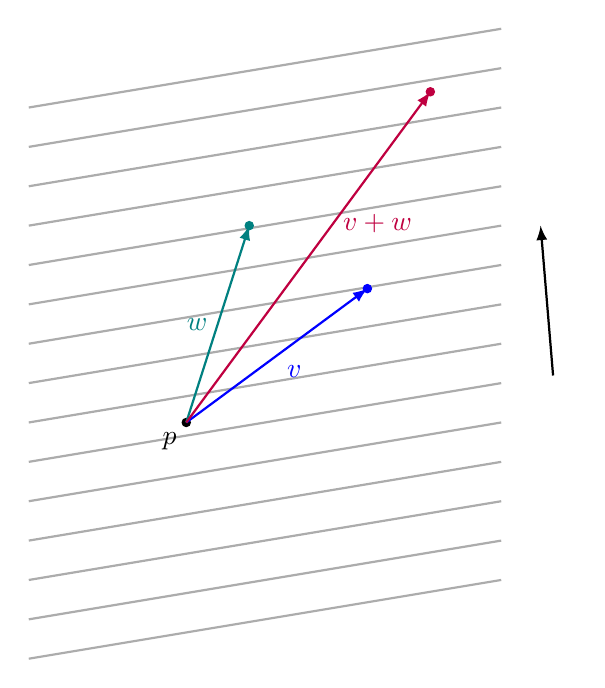
\begin{tikzpicture}[scale=1.0]
    % Diagonal stack lines (visualizing a covector)
    \foreach \k in {-3.5,-3.0,...,3.5} {
        \draw[thick,gray!65] (-3,\k-0.5) -- (3,\k+0.5);
    }
    % Orientation arrow
    \draw[->,thick,black] (3.65862,-0.40344) -- (3.5,1.5);
    % Reference point
    \filldraw[black] (-1,-1) circle (1.5pt) node[below left] {$p$};
    % Invisible path to extend bounding box
    \path (3.65862,-0.40344) ++(0.3,0);
    % Vector v
    \draw[->,thick,blue] (-1,-1) -- (1.3,0.7) node[midway,below right] {$v$};
    % Vector w
    \draw[->,thick,teal] (-1,-1) -- (-0.2,1.5) node[midway,left] {$w$};
    % Vector v + w
    \draw[->,thick,purple] (-1,-1) -- (2.1,3.2) node[pos=0.6,right] {$v+w$};
    % Endpoint markers
    \filldraw[blue] (1.3,0.7) circle (1.5pt);
    \filldraw[teal] (-0.2,1.5) circle (1.5pt);
    \filldraw[purple] (2.1,3.2) circle (1.5pt);
\end{tikzpicture}
\caption{Covector acting on tangent vectors}
\label{fig:parallel_stack_lines}
\end{figure}

\cref{fig:1-form_hyperplanes} shows a similar visualization of a covector.
It is the three-dimensional analogue, replacing the stack lines with a stack of planes.
As we go to higher dimensions, covectors will maintain this geometric interpretation, even though it becomes impossible to visualize (without some tricks).
In general, a covector can be seen as an oriented stack of hyperplanes.
A covector field can be seen as a collection of these stacks of hyperplanes near a point.
For convenience, we will usually refer to the hyperplanes as just lines.

\begin{figure}[!htbp]
    \centering
    \scalebox{1.5}{\includegraphics{1-form_hyperplanes}}
    \captionsetup{justification=centering}
    \caption{Visualization of covectors as hyperplanes
    \\Credits: Maschen -- Own work, \href{https://creativecommons.org/public-domain/cc0/}{CC0}, via Wikimedia Commons}
    \label{fig:1-form_hyperplanes}
\end{figure}

Given two covectors $\alpha_p$ and $\beta_p$, their sum $(\alpha + \beta)_p$, or equivalently $\alpha_p + \beta_p$, can be visualized as combining the two sets of stack lines.
This is simple if they are parallel; the two covectors simply combine into a scalar multiple of one of them.
Otherwise, $(\alpha + \beta)_p$ is represented by the set of stack lines formed by the intersections of the lines of $\alpha_p$ and $\beta_p$.
If the former is a set of stack lines pointing north, and the latter is a set of stack lines pointing east, then there combination will point northeast.

Alternatively, we may visualize the sum as the union of the two sets of stack lines.
Both ways allow us to correctly evaluate tangent vectors by counting how many stack lines they pierce, and both extend to higher dimensions using hyperplanes.
A disadvantage of the second way is that it does not clearly show that the sum of the two covectors is itself a covector.
It is also unfortunately not clear that these two ways represent the same covector simply by looking at them in a diagram.

Now, consider the covector field associated with the function $f(x, y) = x$.
This is shown in \cref{fig:heatmap_x}.
Its contour lines are straight, parallel, and have equal spacing.
They point to the right.
The covector at any point will look identical to the contour lines, except that it will always have unit spacing between stack lines.
A vector that points completely vertically will not cross any stack lines, so its measurement will read zero.
In general, only the $x$-component of a tangent vector will contribute to the measurement.
Due to the unit spacing, the measurement will be exactly the $x$-component of the vector.

\begin{figure}[!htbp]
\centering
\tikzsetnextfilename{heatmap_fx}
\begin{tikzpicture}
\begin{axis}[
    width=10cm,
    height=10cm,
    view={0}{90},
    colormap/jet,
    xlabel={$x$},
    ylabel={$y$},
    colorbar,
    colorbar style={
        ylabel={$f(x,y)$}
    },
    xmin=-10, xmax=10,
    ymin=-10, ymax=10,
    domain=-10:10,
    y domain=-10:10,
]

% Create heatmap with interpolated shading
\addplot3[
    surf,
    shader=interp,
    samples=50,
] 
{x};

% Overlay contour lines showing constant function values
\addplot3[
    contour gnuplot={
        levels={-8,-6,-4,-2,0,2,4,6,8},
        labels=false,
    },
    samples=90,
    samples y=90,
    thin,
    contour/draw color=black,
] {x};

\end{axis}
\end{tikzpicture}
\caption{Plot of $f(x,y) = x$}
\label{fig:heatmap_x}
\end{figure}

Note that (tangent) vectors are objects that do not themselves depend on a chosen coordinate system.
The $x$-component chosen by the aforementioned covector is the first component the vector would have if it were expressed with Cartesian coordinates.
It is the number of parallel, unit-spaced stack lines that would be crossed by the vector.
Covectors are concepts completely independent of coordinates; this is a very important fact.

The covectors associated with $f(x,y) = y$ similarly pick out the $y$-component of a tangent vector.
We have thus found two covector fields whose covectors do completely different things.
Using both of them, we can pick out both parts of a tangent vector.
This strongly suggests that they will form our basis for the cotangent space.
Indeed, the natural choice of basis immediately follows from simply visualizing covectors and considering the simplest cases.

The basis for $T_p \R^2$ will be $\{\d{x}, \d{y}\}$.
These pick out the components of tangent vectors, so $\d{x}(\partial_x) = 1$, $\d{x}(\partial_y) = 0$, $\d{y}(\partial_x) = 0$, and $\d{y}(\partial_y) = 1$.
Generalizing this, the basis for $T^*_p \R^n$ will be $\{\d{x}^1, \ldots, \d{x}^n\}$, with
\begin{equation*}
    \eval{\d{x}^i}{p} \left(\eval{\partial_{x_j}}{p}\right) = \begin{cases}
        1 & \text{if } i = j,\\
        0 & \text{if } i \neq j.
    \end{cases}
\end{equation*}
Here, we have specified that both the covector and tangent vector act at the point $p$ with an evaluation bar.
This is technically the proper way to do it, but it is often omitted, as we did in the paragraph above.
This is done when context makes it clear what (possibly arbitrary) point we are talking about.
Since we very often talk about both covector fields $\omega$ and covectors $\omega_p$, the distinction between them is often made via notation.
For tangent spaces, we use an uppercase letter such as $V$ to distinguish them from tangent vectors $v$; this is needed less frequently.

A general covector $\omega_p$ can be expressed as a linear combination of the basis covectors.
It can be seen as a set of stack lines obtained by a combination of horizontal and vertical stack lines.
\begin{equation*}
    \omega_p = \sum_{i=1}^{n} (\omega_p)_i \d{x}^i
\end{equation*}
A covector field is expressed similarly.
Each component $\omega_i$ is a smooth, scalar-valued function of points $p$ on $M$.
\begin{equation*}
    \omega = \sum_{i=1}^{n} \omega_i \d{x}^i
\end{equation*}
One caveat of this is that we are generally not able to write such an expression for a covector field that is valid for an entire manifold.
It is always valid locally, since any manifold resembles $\R^n$ near a point, but the geometry of the manifold might mean that it is not possible globally.
Since we have decided not to delve too deep into the theory of manifolds, this is not a major problem for us.

Examples of covectors include $\d{x}$, $5 \d{x} + 2\d{y}$, and $\d{x} - 6\d{z}$.
An example of a covector field is $x^2 z \d{x} + 2 \d{y} - y\sin x \d{z}$, where inputting some values for $x$, $y$, and $z$ turns it into a covector.
The way covectors act on basis tangent vectors, and the fact that they are linear, is enough to evaluate any covector at a given tangent vector.
For instance, given $\omega_p = 3 \d{x} + 2 \d{y}$ and $v = 5 \partial_x - \partial_y$, we have
\begin{align*}
    \omega_p(v) &= \omega_p (5 \partial_x - \partial_y) \\
    &= 5 \omega_p (\partial_x) - \omega_p (\partial_y) \\
    &= 5(3 \d{x} + 2 \d{y}) (\partial_x) - (3 \d{x} + 2 \d{y}) (\partial_y) \\
    &= 5 \cdot 3 \d{x}(\partial_x) + 5 \cdot 2 \d{y}(\partial_x) - 1 \cdot 3 \d{x}(\partial_y) - 1 \cdot 2 \d{x}(\partial_y) \\
    &= 15 \cdot 1 + 10 \cdot 0 - 3 \cdot 0 - 2 \cdot 1 \\
    &= 13.
\end{align*}
We did this the long way on purpose.
We split the expression twice, using the fact that covectors are linear maps and that the addition of covectors is linear.
Note that evaluating a covector involves inputting a vector.
Evaluating a covector field involves inputting a point and then a vector.
Thus, they can be thought of as one-step and two-step evaluations, respectively.

Let us apply this and find the cotangent space for a point on the unit circle, $T^*_p \mathbb{S}^1$ (again, not a proof).
Previously, we found that the tangent space $T_p \mathbb{S}^1$ is spanned by the vector
\begin{equation*}
    v = - \sin t_0 \eval{\frac{\partial}{\partial x}}{p} + \cos t_0 \eval{\frac{\partial}{\partial y}}{p},
\end{equation*}
where $t=t_0$ corresponds to p by the parameterization $\gamma \colon [0, 2\pi) \to \mathbb{S}^1$ with $\gamma(t) = (\cos t, \sin t)$.
We get the above vector by differentiating $\gamma$ with respect to $t$, so we can label the basis tangent vector $\partial_t$.
Now, since $T_p \mathbb{S}^1$ is one-dimensional, it makes sense that $T^*_p \mathbb{S}^1$ is also one-dimensional.
Its basis vector will be the covector $\d{t}$, with $\d{t}(\partial_t) = 1$.
We wish to write this covector in the form $\omega_p = A \d{x} + B \d{y}$.
This can be done by simply evaluating $\omega_p$ at $v = \partial_t$.
\begin{equation*}
    \omega_p(v) = \left( A \eval{\d{x}}{p} + B \eval{\d{y}}{p} \right) \left( - \sin t_0 \eval{\frac{\partial}{\partial x}}{p} + \cos t_0 \eval{\frac{\partial}{\partial y}}{p} \right)
\end{equation*}
This time, we will approach this the quick way by simply picking out the components.
\begin{equation*}
    \omega_p(v) = - A \sin t_0 + B \cos t_0 = 1
\end{equation*}
Using the Pythagorean identity for sine and cosine, we see that $A = - \sin t_0$ and $B = \cos t_0$ is a valid solution.
Hence, our basis covector is
\begin{equation*}
    \omega_p = \eval*{\d{t}}{p} = \omega_p(v) = - \sin t_0 \d{x} + \cos t_0 \d{y},
\end{equation*}
and $T^*_p \mathbb{S}^1 = \operatorname{span}\{\eval{\d{t}}{p} \}$.

\section{Integration of Covector Fields}

Now, having provided a sufficient introduction to covectors and covector fields, we will show how they can be integrated.
They were developed for this purpose, and their notation purposefully resembles integrands.
This is especially apparent from our choice in the symbol used to represent basis covectors.\footnote{Our use of upright symbols is an intentional choice to note that these are distinct from the $dx$ used for differentials previously.}
Although pushforwards -- and the more primitive notions of differentials -- looked like integrands, this was more of a superficial resemblance.
We did not have the machinery to go further with any ideas.
Still, we are only able to work with integrating curves, but we will build up from there.

The general idea of integrating a covector field does not differ much at all from how integration of an $\R \to \R$ function works.
Integration is always a way to sum quantities in a `limiting' way; the individual contributions can be thought of as infinitely small.
Given a one-dimensional manifold $C$, which is just a curve, we can integrate a covector field $\omega$ over this.
At some point $p$ on $C$, the field $\omega$ specifies a covector $\omega_p$, which acts on the tangent vector $v \in T_p C$ to give $\omega_p(v)$.
These measurements are accumulated over $C$ to give us the result of an integral.

Since each measurement represents the number of stack lines of a covector that are pierced by a tangent vector (the exact one will be shown not to matter) at that point, the integral will represent the total accumulation of these numbers.
However, we already know that covectors are what the covector field resembles near a point.
It reasonably follows that, when a covector field can be represented as a single, global topographic map, the integral represents the number of contour lines of the covector field that are pierced by the curve $C$ \cite{covector_integration_visualization}.
Otherwise, it still gives meaningful (though, different) geometric information.
Integration takes the local measurements to give an overall, global measurement.

To see how exactly this works and how we can evaluate our integral, we introduce the concept of the \emph{pullback}.
If we could transform our problem of integrating over the curve $C$ to (an interval of) the real line, our job would be done.
We know how to integrate over the latter.
Suppose we have some function $\phi\colon \R \to C$.
We can use this to `pull' the covector from $T_p C$ to $\R$.
How is this done?
We know that the pushforward $D\phi_p$ is a map from $T_p \R$ to $\T_p C$, and the covector $\omega_{\phi(p)}$ is a map from $T_{\phi(p)} C$ to $\R$.
Thus, precomposing $D\phi_p$ with $\omega_{\phi(p)}$ gives us a function $\omega_{\phi(p)} \circ D\phi_p \colon T_p \R \to \R$.

The domain of the inner map and the codomain of the outer maps become the domain and codomain of our composite map.
That is just how composing maps and functions works.
A notation for the pullback we described above is $\phi^*$.
Given its relation to the pushforward, it makes sense that an alternative notation for $D\phi$ is $\phi_*$.
Now, putting this together, we can use some map $\phi$ to pull $\omega$ back to an interval of the real line, which we can integrate over.
Our formula for the integral of $\omega$ over a curve $C$ parameterized by $\gamma: [a,b] \to C$, which decides its orientation, is defined as
\begin{equation*}
    \int_\gamma \omega \coloneq \int_a^b \gamma^* \omega.
\end{equation*}
We need to find an expression for the pullback $\gamma^*\omega$.
Note that $\gamma^*\omega$ at a point $t \in [a,b]$ is given by $\omega_{\gamma(t)} \circ D\gamma_t$.
This is a map from $T_p[a,b]$ to $\R$, making it a covector.
Since we are working with an interval of $\R$ (which is one-dimensional), our covector will be of the form $f(t) \d{t}$.
Now, we must find $f(t)$.
This can be done by inputting any tangent vector into both sides of the equation $\omega_{\gamma(t)} \circ D\gamma_t = f(t) \d{t}$, since the equality is true for all tangent vectors.
The simplest option is the basis tangent vector, $\partial_t$.
On the RHS, we get
\begin{equation*}
    (f(t) \d{t})(\partial_t) = f(t).
\end{equation*}
On the LHS, we first evaluate $D\gamma_t(\partial_t)$ is simply the velocity of the curve, $\gamma'(t)$.
Hence, $(\gamma^*\omega)_t = \omega_{\gamma(t)}(\gamma'(t))$.
Our formula for the integral is therefore
\begin{equation*}
    \int_\gamma \omega = \int_{a}^{b} \omega_{\gamma(t)}(\gamma'(t)) \d{t}.
\end{equation*}
Whilst this could still be considered to be the integral of a covector field (hence the upright $\d{t}$), that was not the problem with our original integral.
The problem was that we were integrating it over some curve.
Now, it perfectly coincides with a standard Riemann integral over $[a,b] \subset \R$.
This means that we have now defined integration over $\omega$ and given it in a form that can be easily evaluated.
As a side note, we will consider all Riemann integrals $\int_a^b f(x) \d{x}$ as the integral of the covector field $f(x) \d{x}$ over $[a,b]$.
This is not doing anything new -- just relabelling.

For our new definition of the integral over a curve to be sensible, it would have to be independent of the way we parameterize the curve.
To show that is indeed the case, consider $\tilde{\gamma} \colon [\alpha, \beta] \to C$ to be another parameterization of $C$.
Then, there is a bijection between $\gamma$ and $\tilde{\gamma}$, $\varphi \colon [\alpha, \beta] \to [a, b]$, such that $\tilde{\gamma}(\tau) = \gamma(\varphi(\tau))$ and $\varphi'(\tau) > 0$.
The last condition was for $\tilde{\gamma}$ to preserve the orientation of $C$ decided by $\gamma$.
The derivative of $\tilde{\gamma}$ is
\begin{equation*}
    \tilde{\gamma}'(\tau) = \gamma'(\varphi(\tau)) \varphi'(\tau).
\end{equation*}
The integral of $C$ using $\tilde{\gamma}$ is
\begin{equation*}
    \int_{\tilde{\gamma}} \omega = \int_{\alpha}^{\beta} \omega_{\tilde{\gamma}(\tau)}(\tilde{\gamma}'(\tau)) \d{\tau} = \int_{\alpha}^{\beta} \omega_{\gamma(\varphi(\tau))}(\gamma'(\varphi(\tau)) \varphi'(\tau)) \d{\tau}.
\end{equation*}
By the linearity of $\omega$,
\begin{equation*}
    \int_{\tilde{\gamma}} \omega = \int_{\alpha}^{\beta} \varphi'(\tau) \omega_{\gamma(\varphi(\tau))}(\gamma'(\varphi(\tau))) \d{\tau}.
\end{equation*}
The substitution $t = \varphi(\tau), \d{t} = \varphi'(\tau) \d{\tau}$ yields (noting the change in limits)
\begin{equation*}
    \int_{\tilde{\gamma}} \omega = \int_{a}^{b} \omega_{\gamma(t)}(\gamma'(t)) \d{t} = \int_\gamma \omega.
\end{equation*}
This means that there is a sensible notion of $\int_C \omega$ given that $C$ has a certain orientation, since all parameterizations of $C$ give the exact same integral.
This is an extremely important fact about covector fields.
They have been chosen as the object to generalize integration precisely because they lend to properties necessary for a definition of integration to make any sense.
If our parameterization $\varphi$ instead reversed the orientation of $C$, so $\varphi(\tau) < 0$, then the calculations above would instead have yielded
\begin{equation*}
     \int_{\tilde{\gamma}} \omega = - \int_{\gamma} \omega,
\end{equation*}
so reversing the direction we integrate along $C$ adds a minus sign to the integral.
This is consistent with our interpretation of the integral.
As long as the curve itself is the same, the number of contour lines crossed by it will be the same.
Since the contour lines have orientation, crossing them in the opposite direction will give the opposite result.
When a global map of contour lines cannot be used, this can instead be visualized by the curve piercing local stack lines.

We can give ourselves physical intuition for the integral of a covector field with the concept of work.
If the covector field represents a force field, $\omega = F_x \d{x} + F_y \d{y} + F_z \d{z}$, then the integral of $\omega$ along a curve $C$ gives the work done along the curve.
Intuitively, this represents how much the force field is aligned with the motion represented by the curve (where the velocity tangent vectors are literal velocities).
Note that the integral of a covector field cannot give the length of a curve by itself.
If we require lengths, then a metric is needed, which is essentially an object that acts as our ruler.
It is additional structure on the manifold.

We will now consider a simple example (we talk about $\gamma$ as being the curve itself in the examples below).
Let $\omega = y\,\d{x} + x\,\d{y}$ be a covector field on $\mathbb{R}^2$, and let the curve be given by $\gamma(t) = (\cos t, \sin t)$ with $t \in [0,\pi]$.
Then,
\begin{equation*}
\gamma'(t) = (-\sin t, \cos t),
\end{equation*}
and
\begin{equation*}
\omega_{\gamma(t)}(\gamma'(t))
= \sin t(-\sin t) + \cos t(\cos t)
= \cos^2 t - \sin^2 t.
\end{equation*}
Therefore,
\begin{equation*}
\int_\gamma \omega = \int_0^\pi (\cos^2 t - \sin^2 t)\,\d{t} = \int_0^\pi \cos(2t)\,\d{t} = 0.
\end{equation*}
Note that we mentioned that $\omega$ is an object on $\R^2$ instead of just on $\gamma$.
This is fine, since a covector field defined on the ambient manifold can be also be considered as an object on the submanifold.
Now, we will compute one more integral which uses a slightly more complicated field.
Let $\omega = (x^2 - y)\,\d{x} + (x + y^2)\,\d{y}$ be a covector field on $\mathbb{R}^2$.
Our curve will be specified by $\gamma(t) = (t, t^2)$ for $t \in [0,1]$.
The derivative is
\begin{equation*}
\gamma'(t) = (1, 2t),
\end{equation*}
so
\begin{equation*}
\omega_{\gamma(t)}(\gamma'(t)) = (t^2 - t^2)(1) + (t + t^4)(2t) = 2t^2 + 2t^5.
\end{equation*}
The integral of $\omega$ along $\gamma$ is thus given by
\begin{equation*}
\int_\gamma \omega
= \int_0^1 (2t^2 + 2t^5)\,\d{t}
= \frac{2}{3} + \frac{1}{3}
= 1.
\end{equation*}
In general, if we have $\omega = f(x) \d{x}$, then the integral along $\gamma \colon [a,b] \to C$ given by $\gamma(t) = x(t)$ is
\begin{equation*}
    \int_\gamma \omega = \int_a^b \gamma^* \omega = \int_a^b f(x(t)) x'(t) \d{t}.
\end{equation*}
That is the same form of an integral that one obtains after preforming a substitution.
We have brought it up to mention that very fact, which will come up again when we further develop our theory.

We have now answered our initial question of what the $dx$ in the integral means, again.
Instead of being an infinitesimal quantity we sum over, it is an object that takes infinitesimals and measures them so that they can be summed.
Precisely, it is a cotangent vector field.
We have provided our fourth and final interpretation of what $dx$ means.
This one has been sought after specifically for its use in integration.
Our work remains incomplete, however.
There is a lot more we can do with our newly developed theory, which is what we will explore in the next section.

\section{Differential Forms}

Currently, we are only able to integrate over one-dimensional manifolds: curves.
This is because a covector takes a single tangent vector and measures it.
This gives us lengths we can sum over, but we need areas in order to integrate over surfaces (two-dimensional manifolds) and volumes in order to integrate over three-dimensional manifolds.
Thus, we need an object that takes multiple tangent vectors as inputs and returns higher-order measurements.
The first step to see what this object could be is to give covectors the new name of one-forms.
Covector fields are given the name of differential one-forms.

At any given point $p$ on a manifold $M$, a differential one-form evaluates to give a one-form, which is a linear functional of the form $T_p M \to \R$.
It reasonably follows that the object that we require is a differential two-form.
This assigns to each point $p$ a two-form, a linear functional $T_p M \times T_p M \to \R$.
Given two tangent vectors, the value of the two-form will represent the signed area of some shape defined by those vectors.
From the fact that areas of objects are always (in some form or another) the product of lengths, it is reasonable to suppose that our two-form is to be constructed from one-forms.
We need to find this construction.

From this point onwards, we will often use the same notation to reference both a two-form and a differential two-form.
That is, the subscript $p$ used for the actual functional is often omitted for the sake of convenience; this is technically an abuse of notation, however.
Due to the properties of the objects we are dealing with, algebraic results for one will be directly related to results for the other.
Context should allow for the distinction between them when it is needed.

Given one-forms $\alpha$ and $\beta$, we will denote the corresponding two-form as $\alpha \wedge \beta$.
This is called a \emph{wedge product}.
As mentioned above, this is an abuse of notation, and the correct notation for the two-form is $(\alpha \wedge \beta)_p$ or $\alpha_p \wedge \beta_p$.
Suppose we have the tangent vectors $u, v, w \in T_p M$.
Let $\omega = \alpha \wedge \beta$, and let $\lambda, \mu \in \R$.
Our two-form must satisfy some properties in order for the result of its evaluation to represent a signed area.
First, it must be linear in both of its inputs.
\begin{itemize}
    \item $\omega (\lambda u + \mu v, w) = \lambda \omega (u, w) + \mu \omega (v, w)$
    \item $\omega (u, \lambda v + \mu w) = \lambda \omega (u, v) + \mu \omega (u, w)$
\end{itemize}
The technical name for this is \emph{bilinearity}.
We also want $\omega(v, v) = 0$, as the area of a line segment should be zero; this makes $\omega$ an \emph{alternating form}.
From these two properties, it follows that
\begin{equation*}
    \omega(u + v, u + v) = \omega(u, u) + \omega(u, v) + \omega (v, u) + \omega (v, v) = 0,
\end{equation*}
so
\begin{equation*}
    \omega(u, v) = - \omega (v, u).
\end{equation*}
Hence, $\omega$ must be \emph{antisymmetric}.
This is enough information to find a suitable object.
The constituent one-forms of $\alpha \wedge \beta$ act on $u$ and $v$ to give us four numbers: $\alpha(u)$, $\beta(u)$, $\alpha(v)$, and $\beta(v)$.
Then, we can consider the vectors $\langle \alpha(u), \beta(u) \rangle$ and $\langle \alpha(v), \beta(v) \rangle$.
We will define the value of our two-form as the area of the parallelogram formed by these two vectors.
It is thus given by the determinant of the matrix formed using the vectors as rows.
\begin{equation*}
    \alpha \wedge \beta (u, v) = \begin{vmatrix}
    \alpha(u) & \beta(u) \\
    \alpha(v) & \beta(v)
    \end{vmatrix}
\end{equation*}
It can be verified via computation that our chosen formula implies that a two-form is an alternating bilinear functional.
Therefore, we have found what we wanted.
To gain better intuition of what a two-form does, consider the simplest example: $\d{x} \wedge \d{y}$.
Whilst $\d{x}, \d{y} \in T^*_p M$ can have any dimension, they must have dimension greater than one if they are to be combined into a two-form.
That is because the tangent vectors in $T_p M$ must have dimension greater than one so that it is possible to construct a parallelogram with them.
Evaluating $\d{x} \wedge \d{y}$ for tangent vectors $u$ and $v$ gives
\begin{equation*}
    \d{x} \wedge \d{y} (u, v) = \begin{vmatrix}
    \d{x}(u) & \d{y}(u) \\
    \d{x}(v) & \d{y}(v)
    \end{vmatrix}
    = \begin{vmatrix}
        u_x & u_y \\
        v_x & v_y
    \end{vmatrix},
\end{equation*}
which is the area of the parallelogram defined by the projection of $u$ and $v$ onto the $xy$--plane.
Note that, if $M$ is two-dimensional, any two-form can be expressed as a scalar multiple of $\d{x} \wedge \d{y}$.
If $\alpha = A\d{x} + B\d{y}$ and $\beta = C\d{x} + D\d{y}$, then (assuming that the wedge product distributes over addition)
\begin{align*}
    \alpha \wedge \beta &= (A\d{x} + B\d{y}) \wedge (C\d{x} + D\d{y}) \\
    &= AC \d{x} \wedge \d{x} + AD \d{x} \wedge \d{y} + BC \d{y} \wedge \d{x} + BD \d{y} \wedge \d{y} \\
    &= AD \d{x} \wedge \d{y} + BC \d{y} \wedge \d{x} \\
    &= (AD - BC) \d{x} \wedge \d{y}.
\end{align*}
In this case, $\alpha \wedge \beta$ evaluates to give a scaled version of the previously-mentioned area.
The vectors $u$ and $v$ in $T_p M$ are mapped to the vectors $\langle \alpha(u), \beta(u) \rangle$ and $\langle \alpha(v), \beta(v) \rangle$ in $\R^2$, which define a parallelogram.
The new parallelogram is the image of the original parallelogram, spanned by $u$ and $v$, under the action of the two-one forms.

An important note to make is that a two-form is not, in general, the wedge product of two one-forms.
It is true for two-dimensional manifolds, since we only have two basis covectors to work with.
They combine in one way to give $\d{x} \wedge \d{y}$.
We will find the same result is true for three-dimensional manifolds.
A generic two-form can be written $\omega = A \d{x} \wedge \d{y} + B \d{x} \wedge \d{z} + C \d{y} \wedge \d{z}$.
Terms such as $\d{x} \wedge \d{x}$ are zero, and terms such as $\d{y} \wedge \d{x}$ are simply negatives of one of three included two-forms.
Any such two-form can be written as the wedge product of two one-forms.

To see why, consider the second diagram in \cref{fig:k-form_hyperplanes}.
This is an extension of the visualization we had for one-forms using hyperplanes.
The wedge product of two one-forms is the intersection of two sets of hyperplanes, along with an orientation.
This forms a grid of tubes, hyperplanes of one fewer dimension.
A two-form in general can be thought of as a grid of tubes -- not necessarily the intersections of hyperplanes.
We can consider the number of intersections made by the parallelogram, defined by two tangent vectors, with these lines as the result of evaluating a two-form.

In three dimensions, the visualization of the wedge products of two one-forms coincides with the visualization of a generic two-form.
Any grid of tubes can be represented by the intersection of two sets of planes.
Hence, for three-dimensional manifolds, any two-form can be expressed as the wedge product of two one-forms.
Consider the case where $M$ is four-dimensional; the tubes are now planes.
Let $\omega = \d{x} \wedge \d{y} + \d{z} \wedge \d{w}$.
This is a combination of a grid of (planar) tubes along the $zw$--plane and a grid of tubes along the $xy$--plane.
They are perpendicular to each other and cannot be expressed as the intersection of two sets of hyperplanes.

Evaluating $\omega$ consists of taking the parallelogram defined by two tangent vectors and counting the number of tubes, which are $(n-2)$-dimensional hyperplanes, crossed in total.
This is equivalent to finding the area of two different scaled parallelograms and summing them together.
For manifolds with dimension greater than three, two-forms are not necessarily the wedge product of two one-forms.
When they are, the two-form is called simple or decomposable.
Since the case of nonsimple two-forms only occurs with four or more dimensions, it is rather difficult to visualize.
It is most accurate to consider them an irreducible combination of what one would imagine as a `regular' grid.

We have now given a proper geometric interpretation of two-forms, explaining the necessary nuance.
A two-form takes two vectors in a tangent space, maps them to possibly multiple parallelograms, and computes the sum of their areas.
This can equivalently be viewed as the two-form being a grid of tubes, counting the number of tubes (in a continuous way) crossed by the parallelogram defined from the two tangent vectors directly.
The actual computation involves calculating the determinant of a matrix.

Our definitions readily extend to forms of higher degree.
Without first thinking about the properties a three-form needs to possess, we can use the wedge product to combine a two-form with a one-form to obtain a three-form.
It will take three tangent vectors as input and is evaluated by computing the determinant of a $3 \times 3$ matrix.
This is the area of a parallelepiped (three-dimensional parallelogram) in $\R^3$.
\begin{equation*}
    \alpha \wedge \beta \wedge \gamma (u, v, w) = \begin{vmatrix}
    \alpha(u) & \beta(u) & \gamma(u) \\
    \alpha(v) & \beta(v) & \gamma(v) \\
    \alpha(w) & \beta(w) & \gamma(w)
    \end{vmatrix}
\end{equation*}
There is no need to distinguish between $(\alpha \wedge \beta) \wedge \gamma$ and $\alpha \wedge (\beta \wedge \gamma)$, since they can be shown to both be equal to the above determinant, i.e. the wedge product is associative.
A three-form is an alternating trilinear functional, which measures three-dimensional manifolds to give volumes.
Once again, a three-form in general is not necessarily simple.
This can be seen when considering dimensions greater than four.
Irrespective of that fact, it always maps three tangent vectors to possibly multiple parallelepipeds and computes the sum of their areas.

The third diagram in \cref{fig:k-form_hyperplanes} shows a visualization of the wedge product of three one-forms.
It is a grid of points in the case of three dimensions, and in general, it is a grid of hyperplanes of two fewer dimensions than the hyperplanes of the one-forms; we can call them threads.
A three-form in general is a grid of these threads -- not necessarily the intersection of hyperplanes.
It is then valid to think of a three-form as counting the number of threads crossed by a parallelepiped formed from the three tangent vectors.

\begin{figure}[!htbp]
    \centering
    \scalebox{1.5}{\includegraphics{k-form_hyperplanes}}
    \captionsetup{justification=centering}
    \caption{Visualization of $k$-forms as hyperplanes
    \\Credits: Maschen -- Own work, \href{https://creativecommons.org/public-domain/cc0/}{CC0}, via Wikimedia Commons}
    \label{fig:k-form_hyperplanes}
\end{figure}

In general, $\omega = \omega_1 \wedge \omega_2 \wedge \cdots \wedge \omega_k$ is called a differential $k$-form.
It assigns to each point the $k$-form $\omega_p$ (also called a $k$-covector, but we will not use this name), which is a multilinear alternating functional that measures $k$-dimensional manifolds.
Being multilinear means it is linear in all its inputs.
The formula for $\omega_p$ is given by the determinant of a certain $k \times k$ matrix, the volume of a $k$-dimensional parallelotope in $\R^k$.
\begin{equation*}
    \omega_p(v_1,\dots,v_n)=\begin{vmatrix}
    \omega_1(v_1) & \omega_2(v_1) & \cdots & \omega_k(v_1)\\
    \omega_1(v_2) & \omega_2(v_2) & \cdots & \omega_k(v_2)\\
    \vdots & \vdots & \ddots & \vdots \\
    \omega_1(v_k) & \omega_2(v_k) & \cdots & \omega_k(v_k)
    \end{vmatrix}
\end{equation*}
The intuition and visualizations all extend to this most general case.
A differential $k$-form defined on an $n$-dimensional manifold $M$ can be visualized by a set of $(n-k)$-dimensional hyperplanes.
They act on $k$ tangent vectors by counting the number of these hyperplanes crossed by the parallelotope formed from the tangent vectors -- equivalent to finding the volume of the parallelotope mentioned above.
There is no standard name for these hyperplanes, though the names of ``tubes'' and ``threads'' we used in the other cases were not particularly standard, either.
We simply took them from what the objects resemble in three-dimensional space.

These are all examples of \emph{differential forms}.
They are the subject of our interest, the object that we have slowly worked towards defining in a way that feels natural.
We started with simple enquiries regarding notation that we are familiar with, and this has led to a few concepts -- with more to come -- that are much more general than what we started with.
Differential forms are a very useful tool for the study of higher-level mathematics.
This includes topics where they are the main tool used, as well as those where they provide additional insights and alternative viewpoints to well-established results.

We will define a zero-form to just be a real number, so a differential zero-form is a smooth function from $M$ to $\R$.
The space of zero-forms is thus $\R$.
The wedge product acts between a differential zero-form and another form just like regular multiplication, e.g. $x\d{x} = x \wedge \d{x}$.
This definition has been provided here without justification, but it should feel reasonable.
Functions are already familiar to us, so there is not much to discuss about them; thus far, we have really just given it an alternative name.
We will later see the usefulness of zero-forms when we introduce further concepts.

Now, we will consider the algebra of differential forms with the wedge product.
We have already taken for granted that the wedge product is associative and distributes over addition.
Additionally, the wedge product is an alternating product, as
\begin{equation*}
    \alpha \wedge \alpha = \begin{vmatrix}
    \alpha(u) & \alpha(u) \\
    \alpha(v) & \alpha(v)
    \end{vmatrix}
    = \alpha(u)\alpha(v) - \alpha(u)\alpha(v) = 0.
\end{equation*}
It is, however, not commutative.
Considering two one-forms $\alpha$ and $\beta$, their wedge product is
\begin{align*}
    \alpha \wedge \beta &= \begin{vmatrix}
    \alpha(u) & \beta(u) \\
    \alpha(v) & \beta(v)
    \end{vmatrix} \\
    &= \alpha(u)\beta(v) - \alpha(v)\beta(u) \\
    &= - (\alpha(v)\beta(u) - \alpha(u)\beta(v)) \\
    &= - \begin{vmatrix}
    \beta(u) & \alpha(u) \\
    \beta(v) & \alpha(v)
    \end{vmatrix} \\
    &= - \beta \wedge \alpha.
\end{align*}
This shows that the wedge product is anticommutative.
The fact that swapping one-forms around in a wedge product introduces a negative sign is useful for simplifying more complicated expressions.
In general, $\gamma \wedge \delta = (-1)^{kl} \gamma \wedge \delta$, where $\gamma$ is a $k$-form and $\delta$ is an $l$-form.
Finally, note the obvious fact that $\lambda \cdot (\alpha \wedge \beta) = (\lambda \alpha) \wedge \beta = \alpha \wedge (\lambda \beta)$ for all $\lambda \in \R$.
This is essentially saying that scalar multiplication is compatible with the wedge product.

One-forms $\omega_p \in T^*_p M$ span a vector space over the field of real numbers, $\R$.
The properties of the wedge product mentioned above mean that one-forms, along with the operations of addition and the wedge product, form what is called an \emph{exterior algebra}.
This is denoted by $\extp T^*_p M$.
An exterior algebra is a vector space with additional structure.\footnote{Familiarity with abstract algebra may allow for one to recognize that an exterior algebra is an associative algebra with the property that the wedge product is alternating.}
Any $k$-form can be obtained by adding and wedging one-forms together, so they are all elements of this exterior algebra.
Fittingly, an alternative name for the wedge product is the exterior product.

The exterior algebra contains forms of different degrees, though we can consider vector spaces containing only one degree.
The $k$-th exterior power of $T^*_p M$ is the vector subspace of $\extp T^*_p M$ spanned by elements of the form $\d{x}^1 \wedge \d{x}^2 \wedge \cdots \d{x}^k$, where $\d{x}^i \in T^*_p M$ for $i \in \{1, 2, \ldots, k\}$.
Technically, each $\d{x}^i$ should have an evaluation bar.
A $k$-form is an element of $\extp^k T^*_p M$.
Since this only requires us to know what a one-form (covector) and wedge product are, it is a concise way of defining $k$-forms in general -- and hence defining differential $k$-forms.

Whilst all $k$-forms are elements of the exterior algebra, note that the exterior algebra contains elements that are not $k$-forms at all.
Examples of these include $1 + \d{x}$ or $2\d{x} - \d{y} \wedge \d{z}$; we have not assigned any meaning to the sum of forms of different degrees.
This is due to the way the space is defined, which itself makes no reference of the familiar $k$-forms.
We may refer to these objects as mixed forms, and they have their uses, but they are not at all relevant to us.
All elements of the exterior powers are valid $k$-forms, however.

Assuming that $M$ has $n$ dimensions, the first exterior power of $T^*_p M$ is spanned by $n$ one-forms.
These are our basis covectors, $\d{x}^i$.
Thus, the dimension of $\extp^1 T^*_p M$ is $n$.
The second exterior power is spanned by the two-forms $\d{x}^i \wedge \d{x}^j$ such that $i < j$.
There are $\binom{n}{2}$ such two-forms, so that is the dimension of $\extp^2 T^*_p M$.
Therefore, in general, the dimension of $\extp^k T^*_p M$ is $\binom{n}{k}$. 
The number of dimensions of the exterior algebra will be the sum of the dimensions of every exterior power.
It is equal to
\begin{equation*}
    \sum_{i=0}^{n} \binom{n}{i} = 2^n.
\end{equation*}
As an example, consider the manifold $\R^4$.
The space of zero-forms is $\R$, as it always is.
The space of one-forms has the span $\{\d{x}, \d{y}, \d{z}, \d{w}\}$.
The space of two-forms has the span $\{\d{x} \wedge \d{y}, \d{x} \wedge \d{z}, \d{x} \wedge \d{w}, \d{y} \wedge \d{z}, \d{y} \wedge \d{w}, \d{z} \wedge \d{w}\}$.
The space of three-forms has the span $\{\d{x} \wedge \d{y} \wedge \d{z}, \d{x} \wedge \d{y} \wedge \d{w}, \d{x} \wedge \d{z} \wedge \d{w}, \d{y} \wedge \d{z} \wedge \d{w}\}$.
Lastly, the space of four-forms has the span $\{\d{x} \wedge \d{y} \wedge \d{z} \wedge \d{w}\}$.
We cannot have a nonzero five-form or one of even higher degree, since that would involve repeating one of the basis covectors.
They would wedge to make zero, so the entire form would be zero.

We may notice that the space of $k$-forms matches with the space of $(4-k)$-forms.
This makes sense, since the binomial coefficient is symmetrical: $\binom{n}{k} = \binom{n}{n - k}$.
However, the idea of $k$-forms and $(n-k)$-forms being dual to each other goes deeper than that.
It turns out that there is a one-to-one correspondence between these, and this is an important fact that will be expanded upon later.

The final part of this section involves us providing an explicit formula for $k$-forms.
It is not at all necessary for understanding the rest of the exposition.
A differential $k$-form $\omega$ can be expressed (local to $p$) as follows, where $\omega_{i_1 i_2 \ldots i_k}$ are smooth, scalar-valued functions of $p$ on $M$.
\begin{equation*}
    \omega = \sum_{1 \leq i_1 < i_2 < \cdots < i_k \leq n} \omega_{i_1 i_2 \ldots i_k} \d{x}^{i_1} \wedge \d{x}^{i_2} \wedge \cdots \wedge \d{x}^{i_k}
\end{equation*}
This is incredibly cumbersome to write, so we can use the multi-index $I = (i_1, i_2, \ldots, i_k)$ to greatly simplify the expression.
\href{https://en.wikipedia.org/wiki/Multi-index_notation}{Multi-index notation} is not required for the understanding of any ideas in this exposition -- only to simplify expressions.
Here, we use a prime symbol ad hoc to denote that we are only summing over increasing multi-indices.
\begin{equation*}
    \omega = {\sum_{\abs{I} = k}}' \omega_I \d{x}^I
\end{equation*}
Then, at any point $p$, the $k$-form $\omega_p$ is given by the following.
\begin{equation*}
    \omega_p = {\sum_{\abs{I} = k}}' (\omega_p)_I \d{x}^I
\end{equation*}

\section{Integration of Differential Forms}

With the theory of differential forms developed, we are ready to apply them to integration.
We have already defined what the integral of a differential one-form -- a covector field -- means.
To reiterate, the integral of a differential one-form $\omega$ over some curve $C$ in $M$, with a certain orientation, is defined by
\begin{equation*}
    \int_C \omega \coloneq \int_a^b \gamma^* \omega = \int_a^b \omega_{\gamma(t)} (\gamma'(t)) \d{t},
\end{equation*}
where $\gamma \colon [a,b] \to C$ is a parameterization of $C$ that preserves its orientation, and $\gamma^* \omega$ is the pullback of $\omega$ by $\gamma$.
The interpretation of this integral is that it is the accumulation of local stack lines, representing covectors, that are crossed by the tangent vectors along the curve.
For certain $\omega$, this can also be viewed as the number of contour lines of $\omega$ crossed by $C$.
At each point on the curve, the one-form takes a tangent vector as input.

Consider an orientated surface $S$, which is a two-dimensional manifold, with the parameterization $\sigma \colon U \subset \R^2 \to S$ that preserves its orientation.
It makes sense that the associated form to integral over will be a differential two-form.
The integral of a differential two-form $\omega$ over the surface $S$ is defined as follows.
\begin{equation*}
    \int_S \omega \coloneq \int_U \sigma^*\omega
\end{equation*}
The form of this definition appears identical to the case of one-forms.
For a one-form $\alpha_p$, its pullback with a map $\phi$ is given by $\alpha_{\phi(p)} \circ D\phi_p$.
Extending this idea to two-forms, the pullback $\sigma^*\omega$ at a point $(u, v) \in U$ acts on tangent vectors $X, Y \in T_{(u,v)} U$ to give
\begin{equation*}
    \omega_{\sigma(u, v)} \circ \extp^2 D\sigma_{(u,v)}(X,Y) = \omega_{\sigma(u, v)}(D\sigma_{(u,v)}(X), D\sigma_{(u,v)}(Y)).
\end{equation*}
Consider the use of the exterior power here to just be a shorthand for the messier expression on the right.
We have used it since technically the composition $\omega_{\sigma(u, v)} \circ D\sigma_{u,v}$ does not make sense as a two-form requires two inputs.
Our two-form is of the form $f(u, v) \d{u} \wedge \d{v}$, since we are working with a subset of $\R^2$.
Thus,
\begin{equation*}
    \omega_{\sigma(u, v)} \circ \extp^2 D\sigma_{(u,v)} = f(u, v) \d{u} \wedge \d{v}.
\end{equation*}
Evaluating the RHS at the basis tangent vectors $\partial_u$ and $\partial_v$ gives us $f(u, v)$.
Doing the same on the LHS gives
\begin{equation*}
    \omega_{\sigma(u, v)} \circ \extp^2 D\sigma_{u,v} (\partial_u, \partial_v) = \omega_{\sigma(u, v)}\left(\frac{\partial \sigma}{\partial u}, \frac{\partial \sigma}{\partial v}\right).
\end{equation*}
Our integral can be expressed as
\begin{equation*}
    \int_S \omega = \int_U \omega_{\sigma(u, v)}\left(\frac{\partial \sigma}{\partial u}, \frac{\partial \sigma}{\partial v}\right) \d{u} \d{v}.
\end{equation*}
Note that the partial derivatives $\partial \sigma/\partial u$ and $\partial \sigma/\partial v$ are tangent vectors in $T_{\sigma(u, v)} S$, and can be precisely defined in the same way we defined velocities of curves.
Simply treating them as regular partial derivatives is fine, and that is how they are used when we actually evaluate the integral.
One may note that these partial derivatives, chosen by our parameterization, encodes the orientation of the surface.
Reversing the orientation adds a negative sign to the integral.
Technically, the above formula should read
\begin{equation*}
    \int_S \omega = \int_U \omega_{\sigma(u, v)}\left(\frac{\partial \sigma}{\partial u}, \frac{\partial \sigma}{\partial v}\right) \d{u} \wedge \d{v},
\end{equation*}
as we are still integrating a two-form.
The difference is that is in a region of $\R^2$, so we may identify it with a regular Riemann integral by definition.
If we were rigorously introducing these concepts, then we would consider partitions and how exactly the integral is defined to be a Riemann integral that can be evaluated.
For our purposes, what we have written is fine and the same identification will apply to the integral of any $n$ form.

Now, we will consider what this integral represents.
As described in the previous section, a two-form can be viewed as a grid of tubes, and sometimes as the intersections of two sets of hyperplanes; this is a visualization, and tubes are not actually present on the surface.
It takes two tangent vectors as input, maps them to possibly multiple parallelograms, and computes the sum of their areas by counting the number of tubes they cross.
The integral of a differential two-form is the accumulation of these values at each point on the surface.
Whilst this is accurate, it does not appear to be very meaningful.

First, make note of the fact that integrals of two-forms are independent of coordinates.
It can be shown that our definition does not depend upon of parameterization, just as we showed for the integral of one-forms.
Whilst this is true for all integrals, the object itself that we are integrating here is coordinate-independent.
Besides this, how does our integral differ from a regular double integral?
The latter can be interpreted as summing infinitesimal areas, $f(x) \diff x \diff y$, over a surface.
Among other things, this can be used to calculate the actual area of a surface.

Without a metric, there is no objective sense of size, so there is no objective area of a surface.
The integral of a two-form can give an `area', but it cannot be considered the `correct' one.
Instead, we call the measurement given by the integral `flux'.
Usually, flux is seen as how much of something flows through the surface, but that requires an ambient space.
When working without such a space, there is not really a better way to view than to use the idea of it counting tubes crossed as me mentioned before.
This is an intrinsic viewpoint, and it can still be applied to cases where we do have a metric to work with.
Flux is useful in physics, which has concepts such as electric and magnetic flux.

We will consider a very simple example of an integral a two-form.
Let $\omega = x\,\d{x} \wedge \d{y}$ be a differential two-form on $\mathbb{R}^2$, and let
\begin{equation*}
S = \{(x,y)\in\mathbb{R}^2 : 0 \le x \le 1,\ 0 \le y \le 1\}
\end{equation*}
with the standard orientation.
Using the identity parameterization $\sigma(x,y) = (x,y)$, we have
\begin{equation*}
\sigma^*\omega = x\,\d{x}\wedge\d{y}.
\end{equation*}
Thus,
\begin{equation*}
\int_S \omega = \int_0^1 \int_0^1 x \d{x}\d{y} = \frac{1}{2}.
\end{equation*}
These computations are not particularly important, though including at least a couple is helpful.
We will do one more.
Let $\omega = (x^2 + y)\,\d{x} \wedge \d{y}$ be a differential two-form on $\mathbb{R}^2$, and let $\sigma(u,v) = (u\cos v,\, u\sin v)$ with $(u,v) \in [0,1]\times[0,\pi/2]$.
The two partial derivatives are
\begin{equation*}
\frac{\partial \sigma}{\partial u} = (\cos v, \sin v), \qquad \frac{\partial \sigma}{\partial v} = (-u\sin v, u\cos v).
\end{equation*}
Evaluating the two-form gives
\begin{equation*}
\omega_{\sigma(u,v)} \left(\frac{\partial \sigma}{\partial u},\frac{\partial \sigma}{\partial v}\right)
= \bigl(u^2\cos^2 v + u\sin v\bigr)
\begin{vmatrix}
\cos v & -u\sin v \\
\sin v & u\cos v
\end{vmatrix}
= u^3\cos^2 v + u^2\sin v.
\end{equation*}
Therefore,
\begin{equation*}
\int_S \omega = \int_0^1 \int_0^{\pi/2} \left( u^3\cos^2 v + u^2\sin v \right)\d{v}\d{u} = \frac{\pi}{16} + \frac{1}{3}.
\end{equation*}
Consider the differential two-form $\omega = f(x,y) \d{x} \wedge \d{y}$ and the surface $S$ parameterized by $\sigma \colon U \to S$, which is given by $\sigma(u, v) = (x(u, v), y(u, v))$.
The integral of $\omega$ over $S$ is
\begin{equation*}
    \int_S \omega = \int_U \sigma^*\omega = \int_U f(x(u, v), y(u, v))
    \begin{vmatrix}
        \partial_u x & \partial_v x \\
        \partial_u y & \partial_v y
    \end{vmatrix} \d{u}\d{v}.
\end{equation*}
Recall the integral of $\omega = f(x) \d{x}$ that we mentioned at the end of the section on the integration of covector fields.
We said that it had the form of an integral one obtains after a substitution -- the same is true here.
Now that we are in two dimensions, we can properly see that the Jacobian determinant $\det(D\sigma)$ is present (the pushforward is essentially the Jacobian).
This normally happens when we perform a change of variables in a regular integral.
The two-form measures areas, and the pulling it back to $\R^2$ with $\sigma$ takes an area scaling factor (the determinant).

We can easily extend the ideas covered to $n$-forms.
A differential form whose degree matches that of the manifold is called a \emph{volume form} or a \emph{top(-dimensional) form}, and we can only integrate volume forms over their respective manifold; how would one integrate non-volume forms?.
The integral of a differential $n$-form $\omega$ over an oriented $n$-dimensional manifold $M$ parameterized by $\varphi \colon D \subset \R^n \to M$, which is orientation preserving, is defined to be
\begin{equation*}
    \int_M \omega \coloneq \int_D \varphi^*\omega = \int_D \omega_{\varphi(u^1, \ldots, u^n)}\left(\frac{\partial \varphi}{\partial u^1}, \ldots, \frac{\partial \varphi}{\partial u^n}\right) \d{u^1} \cdots \d{u^n}.
\end{equation*}
Making use of multi-index notation, the above can be rewritten as follows.
Note that $\d{x^I}$ here means something different to when we used multi-index notation to express a $k$-form with its components.
\begin{equation*}
    \int_M \omega = \int_D \omega_{\varphi(u^I)}\left(\frac{\partial \varphi}{\partial u^I}\right) \d{u^I}
\end{equation*}
Its interpretation is also practically the same.
An $n$-form measures $n$ tangent vectors by converting them into possibly multiple $n$-dimensional parallelotopes and computing the sum of volumes.
The integral accumulates this at every point on the manifold.
It always represents some sort of amount, which is not necessarily a physical volume.
The exact amount it represents depends on the context and can include mass, charge, and probability.
We can get a consistent notion of volumes of manifolds, but they are not canonical without a metric.
It is independent of the parameterization of $M$ -- so coordinate-independent -- and reversing the orientation of the manifold flips the sign of the integral.

Evaluating the integral of the differential $n$-form $\omega = f(x^1, \ldots, x^n)$ on the manifold $M$ parameterized by $\varphi \colon D \to M$, which is given by $\varphi(u^1, \ldots, u^n) = (x^1(u^1, \ldots, u^n), \ldots, \allowbreak x^n(u^1, \ldots, u^n))$, will yield
\begin{equation*}
    \int_M \omega = \int_D \varphi^*\omega = \int_D f(x^1(u^1, \ldots, u^n), \ldots, x^n(u^1, \ldots, u^n)) \det(D\varphi) \d{u^1} \cdots \d{u^n}.
\end{equation*}
We have made the equation rather messy by explicitly showing that $x^1, \ldots, x^n$ take $u^1, \ldots, u^n$ as inputs.
The important part is the Jacobian determinant factor.
This has the exact same interpretation as in the case of two-forms, though now it represents a volume scaling factor.

With this, we have defined integration of differential forms, which was the main goal of this exposition.
After discussing the Riemann integral and considering what the $dx$ meant, we were led down a string of ideas that ended up with the introduction of differential forms.
These are objects whose main purpose is to be integrands.
Not only have they provided a (hopefully) satisfying interpretation of the standard notation found in integrals, they have allowed us to make the vast generalization from integrating over objects in Euclidean space to integrating over smooth manifolds.
There is so much more that we can do with manifolds, which have plenty of applications to other subjects.

Our main objective is finally complete, but the introduction of differential forms entails the further study of the objects themselves and their applications.
In that regard, there is much more left -- far more than what can be covered in an introductory exposition.
Many require us to consider smooth manifolds with additional structure.
Indeed, adding a metric allows us to introduce a variety of new concepts.
We will not do this, and instead stop with two more topics still very much related to the integration of forms.

This exposition was originally formulated, and motivated throughout, with integration in mind.
It is likely beneficial to stick to this in order to maintain a general sense of cohesion.
Another thing to consider is ideas related to differential forms that do not require a metric are those which are truly fundamental to the objects.
Our choice of visualizations and the careful language we have used has been in order to not fall victim to assuming extraneous structure.
This is how we will continue the rest of the way through.

\section{The Exterior Derivative}

So far, we have introduced differential forms, and we have discussed how two such forms may be combined using the wedge product to yield a form of higher degree.
Is there a sensible way of taking a single differential form and converting it to one of higher degree?
What were the caveats relating to the visualization of differential forms on a global scale that we have so far skipped over?
Can we further develop our theory of integration?
How do the major integration theorems of multivariable calculus translate over to the language of manifolds and forms?

These questions are all answered by the introduction of one new concept.
The \emph{exterior derivative} of a smooth function $f \colon M \to N$, denoted $\d{f}$, is the one-form which acts on a tangent vector $v \in T_p M$ in the same way that the pushforward $Df$ does.
\begin{equation*}
    \d{f}(v) \coloneq Df(v) \in T_{f(p)} N
\end{equation*}
As a smooth function can be considered to be a differential zero-form, so the exterior derivative maps zero-forms to one-forms.
In general, it maps $k$-forms to $(k+1)$-forms.
We will arrive at the way it does this by specifying conditions we expect the exterior derivative to satisfy.
Linearity and the Leibniz rule were the defining properties of a derivation, as they generalized the concept of differentiation.
It is reasonable for the exterior derivative to also be linear.
Given that $\alpha$ and $\beta$ are two $k$-forms, and that $\lambda, \mu \in \R$, we have
\begin{equation*}
    \d(\lambda\alpha + \mu\beta) = \lambda\d{\alpha} + \mu\d{\beta}.
\end{equation*}
We also wish for the exterior derivative to satisfy some form of the Leibniz rule.
For derivations $v$, we had $v(fg) = v(f)g + fv(g)$.
The product of smooth functions commutes, $fg = gf$, but the wedge product of forms does not.
Given that $\alpha$ is a $k$-form and $\beta$ is an $l$-form, the antisymmetry of the wedge product gives us
\begin{equation*}
    \alpha \wedge \beta = (-1)^{kl} \beta \wedge \alpha.
\end{equation*}
Taking the exterior derivative on both sides of the equation gives
\begin{equation*}
    \d(\alpha \wedge \beta) = \d((-1)^{kl} \beta \wedge \alpha) = (-1)^{kl} \d(\beta \wedge \alpha).
\end{equation*}
If it were true that $\d(\alpha \wedge \beta) = \d{\alpha} \wedge \beta + \alpha \wedge \d{\beta}$, then it would follow that
\begin{align*}
    \d{\alpha} \wedge \beta + \alpha \wedge \d{\beta} &= (-1)^{kl} \d{\beta} \wedge \alpha + (-1)^{kl} \beta \wedge \d{\alpha} \\
    &= (-1)^{kl} \beta \wedge \d{\alpha} + (-1)^{kl} \d{\beta} \wedge \alpha \\
    &= (-1)^{kl} (-1)^{(k+1)l} \d{\alpha} \wedge \beta + (-1)^{kl} (-1)^{k(l+1)} \alpha \wedge \d{\beta} \\
    &= (-1)^{2kl} (-1)^l \d{\alpha} \wedge \beta + (-1)^{2kl} (-1)^k \alpha \wedge \d{\beta} \\
    &= (-1)^l \d{\alpha} \wedge \beta + (-1)^k \alpha \wedge \d{\beta}.
\end{align*}
This is nonsensical.
If we had this as a defining property of the exterior derivative, then it would simply map all forms to zero.
If we instead require it to satisfy $\d(\alpha \wedge \beta) = \d{\alpha} \wedge \beta + (-1)^k \alpha \wedge \d{\beta}$, then the above algebraic manipulations yield a different result.
\begin{align*}
    \d{\alpha} \wedge \beta + (-1)^k \alpha \wedge \d{\beta} &= (-1)^{kl} \d{\beta} \wedge \alpha + (-1)^{kl} (-1)^l \beta \wedge \d{\alpha} \\
    &= (-1)^{(k+1)l} \beta \wedge \d{\alpha} + (-1)^{kl} \d{\beta} \wedge \alpha \\
    &= (-1)^{(k+1)l} (-1)^{(k+1)l} \d{\alpha} \wedge \beta + (-1)^{kl} (-1)^{k(l+1)} \alpha \wedge \d{\beta} \\
    &= (-1)^{2(kl+l)} \d{\alpha} \wedge \beta + (-1)^{2kl} (-1)^k \alpha \wedge \d{\beta} \\
    &= \d{\alpha} \wedge \beta + (-1)^k \alpha \wedge \d{\beta}.
\end{align*}
We have arrived at a tautology, showing that the modified condition gives the exterior derivative antisymmetry which matches that of the wedge product.
The extra factor of $(-1)^k$ could be considered the cost for $\d$ to move past the $\alpha$ in $\alpha \wedge \beta$.
We say that the exterior derivative must satisfy the \emph{graded Leibniz rule}.
It is a generalization of the product rule to objects which are antisymmetric.
The final condition required to specify the exterior derivative is that it gives zero when applied twice, i.e. $\d^2 = 0$; we may refer to this as \emph{nilpotence}.\footnote{Nilpotence is a more general term, referring to the vanishing of objects when they are applied consecutively some number of times.}
This certainly does not seem as reasonable as the other conditions, though that should change after we reveal the geometric interpretation of the exterior derivative.

First, we will consider some computations.
By the first property, the smooth (coordinate) function $x$ on $M$ turns into the differential one-form $\d{x}$.
The one-form $\d{x}$ turns to $\d{\d{x}} = \d^2{x} = 0$.
It might seem as if the exterior derivative of any one-form is zero.
Certainly, given $\omega = \lambda_1\d{x^1} + \lambda_2\d{x^2} + \cdots + \lambda_k\d{x^k}$, we have $\d{\omega} = 0$ by linearity and nilpotence.
A counterexample is the one-form $\omega = x\d{y} = x \wedge \d{y}$.
The graded Leibniz rule gives us
\begin{equation*}
    \d{\omega} = \d(x \wedge \d{y}) = \d{x} \wedge \d{y} + (-1)^0 x \wedge \d{\d{y}} = \d{x} \wedge \d{y}.
\end{equation*}
Now, recall that the pushforward generalizes the concept of the differential of functions from $\R^n$ to $\R^m$.
Given a certain coordinate basis, they have very similar formulae, though the former acts on tangent vectors.
The pushforward $Df$ of a smooth function $f$, without specifying a particular point $p$ to evaluate at, is given by
\begin{equation*}
    Df(v) = \sum_{i=1}^n \sum_{j=1}^m v^i \frac{\partial f^j}{\partial x^i} \frac{\partial}{\partial y^j},
\end{equation*}
This is simply taken and slightly modified from the section on tangent spaces.
Given that $f$ maps to $\R$, the formula simplifies to
\begin{equation*}
    Df(v) = \sum_{i=1}^n v^i \frac{\partial f}{\partial x^i} \frac{\partial}{\partial y}.
\end{equation*}
The exterior derivative of the zero-form $f$, $\d{f}$, has the same formula as $Df$, except that the partial derivative operators are replaced with the basis covectors.
Note that the presence of a covector implies that the object will act on a tangent vector.
Thus, we can provide the formula for this unambiguously without needing to reference the tangent vector it is acting on.
\begin{equation*}
    \d{f} = \sum_{i=1}^n \frac{\partial f}{\partial x^i} \d{x^i}
\end{equation*}
This is all we need to evaluate the exterior derivative of any differential form.
The two-form $\omega = z \d{x} \wedge \d{y} + 3y^2 \d{x} \wedge \d{z}$ is converted into a three-form as follows.
\begin{align*}
    \d{\omega} &= \d(z \d{x} \wedge \d{y} + 3y^2 \d{x} \wedge \d{z}) \\
    &= \d(z \d{x} \wedge \d{y}) + 3 \d(y^2 \d{x} \wedge \d{z}) \\
    &= \d{z} \wedge \d{x} \wedge \d{y} + 6y \d{y} \wedge \d{x} \wedge \d{z} \\
    &= \d{x} \wedge \d{y} \wedge \d{z} - 6y \d{x} \wedge \d{y} \wedge \d{z} \\
    &= (1 - 6y) \d{x} \wedge \d{y} \wedge \d{z}.
\end{align*}
Note that we have taken some shortcuts above.
First, we have omitted the terms in the product rule that are not from the derivative of a zero-form.
Those omitted terms would all involve $\d^2$, and hence evaluate to zero.
The exterior derivative of $y^2$ is $2y \d{y}$.
Swapping the covectors in the second term introduced a minus sign, since we performed an odd number of swaps; swapping them in the first term preserved the sign.

Note that for smooth functions, the exterior derivative is essentially identical to the pushforward, so it too is a generalization of the regular derivative of functions defined on Euclidean space.
Indeed, given two smooth functions $f$ and $g$, we have $\d(fg) = \d(f \wedge g) = \d{f} \wedge g + (-1)^0 f \wedge \d{g} = g\d{f} + f\d{g}$.
This is identical to the product rule.
It can thus be seen that just as differential forms are the natural way to extend the theory of integration, they are the natural way to extend differentiation.

From our definition of the exterior derivative, which makes use of the properties we expect it to have, we can express $\d{\omega}$ in a somewhat nice formula for any $k$-form $\omega$.
The formula could alternatively be used as a definition for the exterior derivative, and we could derive its already listed properties.
This is likely less sensible than the approach we have taken.
As we have previously shown, a general $k$-form can be expressed using multi-index notation (with the ad hoc prime sum) as follows.
\begin{equation*}
    \omega = {\sum_{\abs{I}=k}}' \omega_I \d{x^I}
\end{equation*}
From the previous note we made about the product rule and the only nonzero terms being those which take the exterior derivative of the zero-form, we have
\begin{equation*}
    \d{\omega} = \d \left({\sum_{\abs{I}=k}}' \omega_I \d{x^I}\right) = {\sum_{\abs{I}=k}}' \d(\omega_I \d{x^I}) = {\sum_{\abs{I}=k}}' \d{\omega_I} \wedge \d{x^I}.
\end{equation*}
We may then replace $\d{\omega_I}$ with its previously given formula.
\begin{equation*}
    \d{\omega} = {\sum_{\abs{I}=k}}' \left( \sum_{j=1}^{k} \frac{\partial \omega_I}{\partial x^j} \d{x^j} \right) \wedge \d{x^I}
\end{equation*}
By applying the distributivity of the wedge product over addition, we can remove the set of brackets.
\begin{equation*}
    \d{\omega} = {\sum_{\abs{I}=k}}' \sum_{j=1}^{k} \frac{\partial \omega_I}{\partial x^j} \d{x^j} \wedge \d{x^I}
\end{equation*}
Even with the use of multi-index notation, our final formula is not the prettiest.
In a sense, it could be simplified further.
Terms where $j \in I$ are redundant, evaluating to zero.
We could -- albeit via the introduction of even further ad hoc notation -- have the basis covectors arranged in the correct order.
It is probably best to stop at the form we have arrived at; expressing $\d{\omega}$ in a nice closed-form expression is beside point of its introduction.

It is with the exterior derivative that we have chosen to provide a clear definition before any actual mention of its visualization.
The reasoning behind this is that it should already feel pretty similar to well-known topics, such as the derivative found in regular calculus.
Out of all the major ideas we have introduced in this exposition thus far, the exterior derivative could be considered to be the most immediate extension of previous concepts.
However, a way to visualize it is important, so that is what we will now introduce.
Fortunately, we have already paved the way for it.

Consider the visualizations of functions as heatmap found in the section on cotangent vectors.
Some covector fields may be considered to be the contour lines of the heatmap, which resemble sets of stack lines at a given point.
This then generalizes to differential forms in general, global objects that resemble forms locally.
However, the question remains: which differential forms may be visualized in this way?
In the case where we have a smooth function $f$, its contour map will represent a one-form, as we have stated before.
The contours are the lines along which the function does not change, so its derivative $\d{f}$ is zero.

Indeed, the stack lines that represent one-forms are along the direction where they are zero, e.g. the stack lines of $\d{x}$ are vertical.
Thus, a differential one-form is represented by its zeroes as well.
The contour lines of $f$ represent the differential one-form $\d{f}$.
Then, it follows that a one-form $\omega$ does not have such a visualization if it cannot be expressed as $\omega = \d{f}$ for some smooth function $f$.
These are one-forms which are not \emph{exact}.
We call one-forms which whose exterior derivative vanishes \emph{closed}.
Since being exact implies it is closed by $\d^2 = 0$, not being closed implies that the form is not exact.
For instance, $\d(x\d{y}) = \d{x} \wedge \d{y}$, so this one-form is not exact.

\begin{figure}[!htbp]
\centering
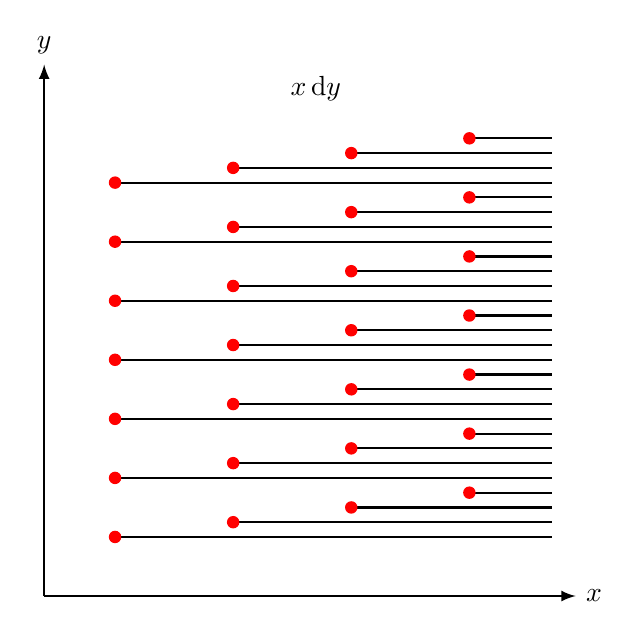
\begin{tikzpicture}[scale=1.5]
    % Draw axes
    \draw[thick, ->] (0,0) -- (4.5,0) node[right] {$x$};
    \draw[thick, ->] (0,0) -- (0,4.5) node[above] {$y$};
    
    % Add label (centered horizontally, high up)
    \node at (2.3,4.3) {$x\d{y}$};
    
    % Draw horizontal lines representing the one-form x dy
    % Density increases with x; lines have staggered left endpoints
    % Each line is continuous from its left endpoint to the right edge
    % Red markers form an evenly spaced grid (spacing 0.5 in y, 1.0 in x)
    \foreach \y in {0.5, 1.0, 1.5, 2.0, 2.5, 3.0, 3.5} {
        % Base line: spans entire width (starts further from y-axis)
        \draw[thick] (0.6,\y) -- (4.3,\y);
        \fill[red] (0.6,\y) circle (1.5pt);
        % Additional lines with staggered left endpoints (increasing density with x)
        \draw[thick] (1.6,\y+0.125) -- (4.3,\y+0.125);
        \fill[red] (1.6,\y+0.125) circle (1.5pt);
        \draw[thick] (2.6,\y+0.25) -- (4.3,\y+0.25);
        \fill[red] (2.6,\y+0.25) circle (1.5pt);
        \draw[thick] (3.6,\y+0.375) -- (4.3,\y+0.375);
        \fill[red] (3.6,\y+0.375) circle (1.5pt);
    }
\end{tikzpicture}
\caption{Visualization of the differential one-form $x\d{y}$}
\label{fig:oneform_xdy}
\end{figure}

We may still visualize it, as is shown in \cref{fig:oneform_xdy}, but it will appear as disjoint collections of constituent one-forms instead of a smooth contour map.
As $x$ increases, the vertical density of the lines increases, which leads to the effect of the lines having endpoints on their left.
The endpoints, which together could be considered the boundary of $x\d{y}$, are present because it is not exact.
We have marked the endpoints in red, and it can be seen that they represent the differential two-form $\d{x} \wedge \d{y}$.
Following the observed rules in the section on differential forms, describing how these visualizations work, we have an evenly spaced grid of points.
Each point itself represents a two-form (points are hyperplanes with $2 - 2 = 0$ dimensions).

The fact that the exterior derivative of the differential form $x\d{y}$ is represented by a boundary is important.
This is something that is true in general.
The exterior derivative $\d{\omega}$ is represented by the boundary of $\omega$.
Although it does not make too much sense to think of the one-form $\d{f}$ as the boundary of the function $f$, considering it as such is useful.
In the case where the form is already the boundary of something, so $\omega = \d{\alpha}$, then $\d{\omega} = \d{\d{\alpha}} = 0$; a boundary does not itself have a boundary.
That is our geometric reason for defining the exterior derivative with the property $\d^2 = 0$.

The concept of exact and closed forms can be extended to differential forms in general.
A differential $k$-form $\omega$ is exact if it can be expressed as $\omega = \d{\alpha}$ for some $(k-1)$-form.
It is closed if $\d{\omega} = 0$.
By nilpotency, all exact differential forms are closed.
Is the converse of this statement -- ``all closed differential forms are exact'' -- true?
The answer to this depends on the nature of the space we are working with.
We will present the following counterexample.
Consider $\R^2 \setminus \{0\}$, the plane with a hole at the origin, and consider along with it the differential one-form $\d{\theta}$ given by
\begin{equation*}
    \d{\theta} \coloneq -\frac{y}{x^2 + y^2} \d{x} + \frac{x}{x^2 + y^2} \d{y}.
\end{equation*}
Here, $\theta$ can be thought of as the phase of a point in the plane, starting at the $x$-axis and going anticlockwise.
It is technically not a function, as the phase of a point $p$ may be $\theta$, or $\theta + 2\pi$, or $\theta + 4\pi$, etc.
We can turn it into a function by assigning to each point a single phase, but it will not be globally consistent.
Suppose $\theta \in [0, 2\pi)$.
Points on the line have a phase of zero, but points directly below have a phase close to $2\pi$.
A loop that starts at the point with $\theta = 0$ and moves around the origin anticlockwise back to that point will pick up a phase of $2\pi$.
More precisely,
\begin{equation*}
    \oint_C \d{\theta} = 2\pi,
\end{equation*}
where $C$ is such a closed loop, e.g. the unit circle.
It is important to note that this only occurs if the loop includes the unit circle.
Otherwise, the values given by $\d{\theta}$ in one direction cancel out with those in the other direction to give an overall accumulation of zero.
As we cannot find a smooth, well-defined function $\theta$, the differential one-form $\d{\theta}$ cannot be expressed as the exterior derivative of such a function.
It is not exact.
However, it can be shown via a quick computation that $\d{\theta}$ is closed.
\begin{align*}
    \d(\d{\theta}) &= \d\left(-\frac{y}{x^2 + y^2} \d{x} + \frac{x}{x^2 + y^2} \d{y}\right) \\
    &= -\d\left(\frac{y}{x^2 + y^2} \d{x}\right) + \d\left(\frac{x}{x^2 + y^2} \d{y}\right) \\
    &= -\d\left(\frac{y}{x^2 + y^2}\right) \wedge \d{x} + \d\left(\frac{x}{x^2 + y^2}\right) \wedge\d{y} \\
    &= -\frac{\partial}{\partial x} \frac{y}{x^2 + y^2}\d{x} \wedge \d{x} -\frac{\partial}{\partial y} \frac{y}{x^2 + y^2} \d{y} \wedge \d{x} \\
    &\phantom{=} + \frac{\partial}{\partial x}\frac{x}{x^2 + y^2} \d{x} \wedge \d{y} + \frac{\partial}{\partial y}\frac{x}{x^2 + y^2} \d{y} \wedge \d{y} \\
    &= -\frac{\partial}{\partial y} \frac{y}{x^2 + y^2} \d{y} \wedge \d{x} + \frac{\partial}{\partial x}\frac{x}{x^2 + y^2} \d{x} \wedge \d{y} \\
    &= \left(\frac{\partial}{\partial x}\frac{x}{x^2 + y^2} + \frac{\partial}{\partial y} \frac{y}{x^2 + y^2} \right) \d{x} \wedge \d{y} \\
    &= \left(\frac{y^2 - x^2}{x^2 + y^2} + \frac{x^2 - y^2}{x^2 + y^2}\right) \d{x} \wedge \d{y} \\
    &= 0
\end{align*}
This shows that it is not always the case that a closed form is exact.
It happens as a result of holes that a space may have, such as the punctured plane in our example.
As (topological) information about a manifold leads to this difference between closed and exact forms, it is reasonable that we can work the other way and use the nature of differential forms to obtain information about a manifold.
When this idea is fully realized, we arrive at \href{https://en.wikipedia.org/wiki/De_Rham_cohomology}{De Rham cohomology}, though it is certainly beyond the scope of this exposition.

We will return to the idea of integration.
We have already learnt how to integral any differential form, but there is much more to the theory than that.
First, we ought to consider the significant results in regular calculus and think of how they may be generalized.
The most important or, perhaps more aptly, fundamental result in single-variable calculus is the fundamental theorem of calculus.
The first part of the theorem relates a function to its definite integrals, and the second part relates definite integrals to indefinite integrals or antiderivatives.
Without mentioning the appropriate conditions, we present the first part as $F'(x) = f(x)$ over $[a, b]$, where
\begin{equation*}
    F(x) \coloneq \int_a^x f(t) \diff t.
\end{equation*}
The second part is presented as
\begin{equation*}
    \int_a^b f(x) \diff x = F(b) - F(a),
\end{equation*}
where $F$ is the antiderivative of $f$, i.e. $F'(x) = f(x)$.
This can be rewritten to include derivatives.
\begin{equation*}
    \int_a^b f'(x) = f(b) - f(a)
\end{equation*}
The importance of these results comes from the fact that they relate the two core concepts of calculus together, when they otherwise may seem completely different.
For someone who is first learning calculus, it is completely reasonable to wonder how the gradients of (tangents to) curves may be related to the areas under curves.
They are in fact very related, and can be considered the inverses of each other.
We will later provide a slightly different way to view the fundamental theorem of calculus.

When we move to the study of multivariable calculus, more theorems are introduced.
Henceforth, we will continue to use the convention of regular letters even for vector functions.
Instead of a function from $\R$ to $\R$, we may have a function from $\R^n$ to $\R$, and it would be called a scalar field.
Just as one has derivatives of real functions, there exists the notion of the gradient of scalar fields.
In $\R^3$, using Cartesian coordinates, the gradient of a scalar field $\varphi$ is a vector field $\nabla \varphi$ given by
\begin{equation*}
    \nabla \varphi = \frac{\partial \varphi}{\partial x} \ihat + \frac{\partial \varphi}{\partial y} \jhat + \frac{\partial \varphi}{\partial z} \khat.
\end{equation*}
In $\R^n$, using Cartesian coordinates, it is given by
\begin{equation*}
    \nabla \varphi = \sum_{i=1}^{n} \frac{\partial \varphi}{\partial x^i} \ehat_i.
\end{equation*}
The integral $\nabla \varphi$ along a smooth curve $\gamma$ which starts at $\mathbf{p}$ and ends at $\mathbf{q}$ is specified entirely by the value of $\varphi$ at the endpoints.
\begin{equation*}
    \int_\gamma \nabla \varphi (\mathbf{r}) \cdot d\mathbf{r} = \varphi(\mathbf{q}) - \varphi(\mathbf{p})
\end{equation*}
This is called the \emph{gradient theorem} or the \emph{fundamental theorem of calculus for line integrals}.
A corollary of this result is that the integral of $\nabla \varphi$ along a closed loop $C$ is zero.
\begin{equation*}
    \oint_C \nabla \varphi (\mathbf{r}) \cdot d\mathbf{r} = 0
\end{equation*}
The scalar field $\varphi$ may be interpreted as a potential, in which case the negative gradient $-\nabla \varphi$ is a conservative force field.
The line integral represents the work done by the force field along a curve, so the work done by conservative forces (such as Newtonian gravity) is path independent.
This is opposed to nonconservative forces such as friction.

Another way to view scalar fields is as giving the elevation of every point in some region, with the gradient giving both the steepness of the region and the direction of steepest ascent at each point.
The interpretation of the gradient theorem in this context is that the difference in elevation between two points does not depend on the path between them.
Indeed, this is the reasoning used when introducing integration of covector fields.
It is also the case that the gradient $\nabla \varphi$ looks exactly like the exterior derivative $\d{\varphi}$ if the unit vectors are replaced with their corresponding covectors.

This relationship between the gradient and the exterior derivative can be made via the introduction of new concepts that require additional structure on a smooth manifold.
As a discussion of such structure is just slightly beyond the scope of this exposition, we will not be able to precisely state the link.
We can still reasonably consider the gradient and the exterior derivative of a function to be essentially the same, so the gradient theorem amounts to the statement that the integral of the derivative of a function $f$ over a curve $\gamma$ with endpoints $a$ and $b$ is
\begin{equation*}
    \int_\gamma \d{f} = f(b) - f(a).
\end{equation*}
By the definition of the integral,
\begin{align*}
    \int_\gamma \d{f} &= \int_a^b \d{f_{\gamma(t)}}(\gamma'(t)) \d{t} \\
    &= \int_a^b \sum_{i=1}^n \frac{\partial f}{\partial x^i}(\gamma(t))\frac{d\gamma^i}{dt} \d{t} \\
    &= \int_a^b \frac{d}{dt} f(\gamma(t)) \d{t} \\
    &= f(b) - f(a).
\end{align*}
Another, perhaps simpler, way of viewing this is that the exterior derivative and the pullback commute.
Using this fact, we can show the above result without needing to expand the derivative.
The exterior derivative is not dependent on coordinates, and the pullback can be viewed as a coordinate transformation, so it makes sense that we could perform the transformation before or after the derivative.
More important for us is the result itself.
The exterior derivative can be used to generalize the gradient theorem, and by extension, the fundamental theorem of calculus.

There is no need to stop at the gradient.
The next integral theorem in multivariable calculus is \emph{Green's theorem}.
The integral of the two-dimensional curl of a function $f$ over an oriented closed curve $C$ is
\begin{equation*}
    \int_C \nabla \times f \diff A = \int_{\partial C} f \cdot \diff \mathbf{r},
\end{equation*}
where $\partial C$ is the boundary of $C$.
Usually, the term on the RHS is written out explicitly, and the notation for the curl is reserved for the actual, three-dimension curl.
However, their interpretation of representing the rotation or circulation of a vector field remains the same, so it makes sense to extend it to this situation.

Then, we have the \emph{curl theorem} or \emph{Stokes' theorem} (latter name not to be confused with a result to come).
The integral of the actual curl of a function $f$ over an oriented surface $S$ with boundary $\partial S = \Gamma$ is given by
\begin{equation*}
    \int_S \nabla \times f \cdot d\mathbf{S} = \int_{\partial S} f \cdot d\mathbf{r}.
\end{equation*}
The fact that this looks so similar to Green's theorem is no coincidence.
We are just taking the surface from two dimensions to a higher-dimensional ambient space; everything else remains the same.
Finally, we have the \emph{divergence theorem}.
The integral of the divergence of $f$ over an oriented volume $V$ is given by
\begin{equation*}
    \int_V \nabla \cdot f \diff V = \int_{\partial V} f \cdot \mathbf{\hat{n}} \diff S.
\end{equation*}
Perhaps, a similarity between these results may be noticed.
With the ones that explicitly present the boundary of the object, it should be more clear.
The integral of some (differential) operator applied to a function over an $n$-dimensional object is equal to the integral of the function itself over the $(n-1)$-dimensional boundary of that object.
If we look closely, and shift our perspective, this is the case for the fundamental theorem of calculus as well.
It can be rewritten as the following equation.
\begin{equation*}
    \int_{[a,b]} f'(x) \diff x = \int_{\partial [a,b]} f(x) \diff x
\end{equation*}
The boundary of the interval $[a, b]$ is the set containing is endpoints (with the correct orientation), and we are considering integrating over it to take the difference between the function applied at those endpoints.
We have relabelled different parts of the equation in order for it to fit the form of the other results.

The exterior derivative applied to a single-variable functions acts just like the ordinary derivative.
Whilst we need extra structure to form a proper equation relating the exterior derivative to the curl and divergence, they can essentially be considered the two- and three-dimensional versions of the exterior derivative, respectively.
The gradient, curl, and divergence are all differential operators, but when one learns about them for the first time in multivariable calculus, they do not possess the necessary knowledge to see them as versions of the same object.

We have unified the integral theorems, and unification implies that there is a single, more abstract way to represent our ideas.
This generalization is called the \emph{generalized Stokes' theorem}.
It may also be called Stokes' theorem on manifolds.
The integral of a differential $n$-form $\omega$ over the boundary of an oriented $n$-dimensional manifold $M$ is equal to the integral of the exterior derivative of $\omega$ over $M$.
This can be put into a very elegant equation.
\begin{equation*}
    \int_{\partial M} \omega = \int_M \d{\omega}
\end{equation*}
This will not be proved, but it should feel like a natural extension of all the previous results.
It encapsulates the ideas we had, extending them to higher dimensions and to much more general objects.
As with many instances of abstractions, the process and end result yields something from which we can further study the objects in question.
In this case, it shows us a connection between the boundary and the derivative.
They are opposites.
They are `dual' to each other.
The fact that the exterior derivative is related to boundaries of forms hinted at this, though we can take our geometrical interpretation further.

We can view $\int_M \d{\omega}$ as counting the lines of $\d{\omega}$ crossed, which make the boundary of the lines of $\omega$.
The only parts of $\omega$ that are not crossed in one way and then the other are those on the boundary.
Hence, we have an equality.
Alternatively, the integral takes the accumulation of the infinitesimal changes in $\omega$, given by $\d{\omega}$, throughout the manifold $M$.
These changes have a direction, and thus they cancel out with each other.
The theorem is thus stating that the only parts that are not cancelled are those on the boundary, which makes sense.
What is left over are the values of $\omega$ on the boundary.

The generalized Stokes' theorem may be regarded as one of the most important results in calculus.
From it comes the fundamental theorem of calculus and the multiple integral theorems of multivariable calculus.
It is all packaged into an idea that can, at least intuitively, be understood very easily.
The integral of the derivative is equal to the integral along the boundary.
There are caveats to consider, but we can appreciate its core idea.
The presentation and explanation of this theorem is likely the best place to end this exposition.

\section{Conclusion}

With the desire to find out what the $dx$ symbol in the integral meant, we first introduced the idea of the differential of a function.
This seemed to define $dx$ and $dy$ independently of their presence in the Leibniz notation for the derivative.
It was a natural way to define them, and differentials certainly have their uses.
However, they did not seem to work with integration, and that is what we really wanted.
For that, we required the differential form, but forms need cotangent spaces.
Cotangent spaces need tangent spaces, and tangent spaces need manifolds.
Hence, we had to start with manifolds.

Our treatment of manifolds was absolutely not a proper indication of their full generality.
After all, our aim was to introduce differential forms, and not the entire subject of differential geometry.
Some details were able to be handwaved as we could focus on the intuition behind the subjects of our study.
Visualization was a key focus in it all.
At this level, with a general lack of rigour, that which can be imagined is valuable.
The methods of visualizing forms and related concepts is really a compilation of what is given by many different sources, all helpful, though none entirely complete.

\section{Resources}

\textsc{Tensor Calculus 6: Differential Forms are Covectors by eigenchris} \, \url{https://www.youtube.com/watch?v=XGL-vpk-8dU}

\textsc{Differential Forms by Michael Penn} \, \url{https://youtube.com/playlist?list=PL22w63XsKjqzQZtDZO_9s2HEMRJnaOTX7}

\textsc{Intro to differential forms by David Metzler} \, \url{https://www.youtube.com/playlist?list=PLB8F2D70E034E9C29}

\textsc{A Geometric Approach to Differential Forms by David Bachman (arXiv version 1)} \, \url{https://arxiv.org/pdf/math/0306194v1}

\textsc{Mathematics Stack Exchange: How to visualize 1 -forms and p -forms?} \, \url{https://math.stackexchange.com/questions/1078427/how-to-visualize-1-forms-and-p-forms}

\textsc{On the Visualisation of Differential Forms by Dan Piponi} \, \url{http://yaroslavvb.com/papers/notes/piponi-on.pdf}

\textsc{On the Visualization of Differential Forms by Duarte Maia} \, \url{https://math.uchicago.edu/~dmaia/documents/visualizing_diff_forms.pdf}

\printbibliography


\begin{appendices}
\crefalias{section}{appsec}
\crefalias{subsection}{appsec}

\section{Vectors} \label{appendix:vectors}

\subsection{Definition of a Vector} \label{appendix:vector_space}

A vector space over a field $\mathbb{F}$ (e.g. $\R$ or $\C$) is a set $V$, along with a binary operation $+ \colon V \times V \to V$, and the operation of scalar multiplication $\cdot \colon \mathbb{F} \times V \to V$, which satisfies the following axioms.
Here, $\mathbf{u}, \mathbf{v}, \mathbf{w} \in V$, and $\lambda, \mu \in \mathbb{F}$.
\begin{enumerate}
\item $\mathbf{u} + \mathbf{v} = \mathbf{v} + \mathbf{u}$
\item $\mathbf{u} + (\mathbf{v} + \mathbf{w}) = (\mathbf{u} + \mathbf{v}) + \mathbf{w}$
\item $\mathbf{0} + \mathbf{v} = \mathbf{v}$
\item $-\mathbf{v} + \mathbf{v} = \mathbf{0}$
\item $\lambda(\mu\mathbf{v}) = (\lambda\mu)\mathbf{v}$
\item $1\mathbf{v} = \mathbf{v}$
\item $\lambda(\mathbf{v} + \mathbf{w}) = \lambda\mathbf{v} + \lambda\mathbf{w}$
\item $(\lambda + \mu)\mathbf{v} = \lambda\mathbf{v} + \mu\mathbf{v}$
\end{enumerate}
The space may be denoted by the tuple $(V, +, \cdot)$, though the associated set $V$ is often used alone.

\subsection{Vector Calculus} \label{appendix:vector calculus}

Defining vectors is itself not the most fruitful task.
A proper definition of real numbers is both motivated and immediately succeeded by a discussion on how to do calculus with them.
We wish to extend those notions to vectors, and we will find that our definitions are not terribly different.
First, consider the simplest case of a vector-valued function whose domain is $\R$.
Let the function be called $\mathbf{f}$ and let $\mathbf{y} = \mathbf{f}(x)$.
There is nothing stopping us from putting this into the regular definition of the derivative.
\begin{equation*}
    \mathbf{f}'(x) = \frac{d\mathbf{y}}{dx} = \lim_{h \to 0} \frac{\mathbf{f}(x+h) - \mathbf{f}(x)}{h}
\end{equation*}
This works perfectly, so we will have it as the definition of the derivative of $\mathbf{f}$ at a point $x$, provided the limit exists.
How do we actually evaluate this derivative?
For that, consider $\mathbf{f}(x) = a(x)\ihat + b(x)\jhat$.
Putting this into our definition gives the following.
\begin{align*}
    f'(x) &= \lim_{h \to 0} \frac{a(x+h)\ihat + b(x+h)\jhat - (a(x)\ihat + b(x)\jhat)}{h} \\
    &= \lim_{h \to 0} \frac{a(x+h) - a(x)}{h}\ihat + \lim_{h \to 0} \frac{b(x+h) - b(x)}{h}\jhat \\
    &= a'(x)\ihat + b'(x)\jhat
\end{align*}
In general, we can differentiate such functions by differentiating their components.
If instead, we consider a function $f$ which maps from $\R^n$ to $\R$ (a vector to a real number), our job becomes much more difficult.
Our regular definition of a limit will not work, as we have to consider vectors approaching other vectors.
Fortunately, it is not too different from the normal $\varepsilon$--$\delta$ definition.
We say that
\begin{equation*}
    \lim_{\mathbf{x} \to \mathbf{a}} f(\mathbf{x}) = \mathbf{L}
\end{equation*}
if and only if, for all $\varepsilon > 0$, there exists a $\delta > 0$ such that for all $\mathbf{x}$ in the domain of $f$,
\begin{equation*}
    0 < \norm{\mathbf{x} - \mathbf{a}} < \delta \implies \norm{f(\mathbf{x}) - \mathbf{L}} < \varepsilon.
\end{equation*}
This simplifies down to the regular definition when $n=1$, and intuitively represents the exact same idea.
The problem arises when we try to generalize differentiation.
For $n=1$, it involves a limit of a fraction, where we divide by $h$.
However, if $n > 1$, then we now have the vector $\mathbf{h}$, and we do not know how to divide by vectors.
We could attempt to resolve it by instead dividing by $\norm{\mathbf{h}}$, saying that the derivative of $f$ at $x$ is
\begin{equation*}
    \lim_{\mathbf{h} \to \mathbf{0}} \frac{f(\mathbf{x}+\mathbf{h}) - f(\mathbf{x})}{\norm{\mathbf{h}}},
\end{equation*}
when this limit exists.
The problem is that, when $n=1$, the limit simplifies to
\begin{equation*}
    \lim_{h \to 0} \frac{f(x+h) - f(x)}{\abs{h}}.
\end{equation*}
Suppose $f(x) = x$.
Our limit becomes
\begin{equation*}
    \lim_{h \to 0} \frac{h}{\abs{h}}.
\end{equation*}
This limit does not exist, meaning that $f(x)$ is not differentiable anywhere under this definition.
Furthermore, it would suggest that $f(x) = \abs{x}$ is differentiable at $x=0$, which is also not true.
Generally, this limit exists only if it is equal to zero.
This is because a limit exists if and only if both the left- and right-hand limits exist.
When $h \to 0^+$, $\abs{h} = h$.
When $h \to 0^-$, $\abs{h} = -h$.
The two one-sided limits differ by their sign, so they are equal only if they are zero.
Although, we can take our original definition of the derivative and move $f'(x)$ inside the limit to get
\begin{equation*}
    \lim_{h \to 0} \frac{f(x+h) - f(x) - hf'(x)}{h} = 0.
\end{equation*}
That is, the derivative of $f$ at $x$ if there is some number $f'(x)$ that satisfies the above statement.
Now, replacing $h$ with $\abs{h}$ will not make a difference.
That means we can generalize our derivative for any $n$.
The derivative of a function $f$ at $\mathbf{x}$ is equal to $D$ if it satisfies
\begin{equation*}
    \lim_{\mathbf{h} \to \mathbf{0}} \frac{f(\mathbf{x}+\mathbf{h}) - f(\mathbf{x}) - D\mathbf{h}}{\norm{\mathbf{h}}} = \mathbf{0}.
\end{equation*}
We may write $D$ as $f'(\mathbf{x})$.
It is important to know what kind of object $D$ is.
It cannot be a real number, since that would make $D\mathbf{h}$ a vector, and the rest of the numerator is a scalar.
If we treat $\mathbf{h}$ as a column vector, then $D$ is a row vector -- their product is a $1 \times 1$ matrix which can be associated with a scalar.
This makes $D$ a $1 \times n$ matrix.
The name for it is the \emph{Jacobian matrix}, or just the Jacobian, and notation for it includes $\mathbf{J_f}(\mathbf{x})$ (the subscript denotes the function it is for) and $\mathbf{J}(\mathbf{x})$.
We can also consider $\mathbf{J_f}$ to be a matrix of functions of $\mathbf{x}$.

Now that we have introduced matrices, we can use them to make the final generalization to functions $\mathbf{f}$ that map from $\R^n$ to $\R^m$ (vectors to vectors).
It follows from everything we have discussed so far that the derivative of $\mathbf{f}$ at $\mathbf{x}$ is an $m \times n$ matrix $\mathbf{J_f}(\mathbf{x})$ if it satisfies
\begin{equation*}
    \lim_{\mathbf{h} \to \mathbf{0}} \frac{\mathbf{f}(\mathbf{x}+\mathbf{h}) - \mathbf{f}(\mathbf{x}) - \mathbf{J_f}(\mathbf{x})\mathbf{h}}{\norm{\mathbf{h}}} = \mathbf{0}.
\end{equation*}
An $m \times n$ matrix multiplied by an $n \times 1$ matrix gives an $m \times 1$ matrix or an $m$-dimensional column vector (the same as the rest of the numerator).
Note that, since a derivative is a matrix, it is a linear map from $\R^n$ to $\R^m$.
This is in-line with the one-dimensional case.
We can then go on to develop familiar concepts with our generalized derivative.
For example, a function is differentiable if there exists some value of $\mathbf{J_f}(\mathbf{x})$ such that the above limit equals $\mathbf{0}$; a function being differentiable implies it is continuous.

One problem we have is that our definition of the derivative is not explicit.
It states that $\mathbf{f}'(\mathbf{x}) = \mathbf{J_f}(\mathbf{x})$ given that $\mathbf{J_f}(\mathbf{x})$ satisfies some condition, but it does not tell us how we actually find the Jacobian.
This in contrast to the case of $n=m=1$, where finding the derivative involves evaluating a limit -- with the function being differentiable if the limit exists.
To find an explicit formula for the derivative, we will first introduce a new concept: the \emph{directional derivative}.
Intuitively, it tells you the rate of change of a function in some particular direction (multiplied by a number).

First, we will start with a function $\mathbf{f}$ from $U$ to $\R^m$, with $U \subseteq \R^n$.
Assume that $\mathbf{f}$ is differentiable at some point $\mathbf{x}$.
Let $\mathbf{v}$ be a fixed element of $\R^n$, and have $\mathbf{h} = t\mathbf{v}$ with $t$ being real.
Since $\mathbf{f}$ is differentiable, we have
\begin{equation*}
    \lim_{t\mathbf{v} \to \mathbf{0}} \frac{\mathbf{f}(\mathbf{x}+t\mathbf{v}) - \mathbf{f}(\mathbf{x}) - t\mathbf{J_f}(\mathbf{x})\mathbf{v}}{\norm{t\mathbf{v}}} = \mathbf{0},
\end{equation*}
assuming $\mathbf{v} \neq \mathbf{0}$.
This can be rewritten as
\begin{equation*}
    \lim_{t \to 0} \frac{\mathbf{f}(\mathbf{x}+t\mathbf{v}) - \mathbf{f}(\mathbf{x}) - t\mathbf{J_f}(\mathbf{x})\mathbf{v}}{\abs{t}\norm{\mathbf{v}}} = \mathbf{0}.
\end{equation*}
Since $\mathbf{v}$ is fixed (does not depend on $t$), we get
\begin{equation*}
    \lim_{t \to 0} \frac{\mathbf{f}(\mathbf{x}+t\mathbf{v}) - \mathbf{f}(\mathbf{x}) - t\mathbf{J_f}(\mathbf{x})\mathbf{v}}{\abs{t}} = \mathbf{0},
\end{equation*}
which is equivalent to
\begin{equation*}
    \mathbf{J_f}(\mathbf{x})\mathbf{v} = \lim_{t \to 0} \frac{\mathbf{f}(\mathbf{x}+t\mathbf{v}) - \mathbf{f}(\mathbf{x})}{t}.
\end{equation*}
The final statement is also true for $\mathbf{v} = \mathbf{0}$, so it is true for all $\mathbf{v}$.
This limit is of the same form as the derivative for $n=1$, as it gives an explicit value of the Jacobian applied to any vector $\mathbf{v}$.
However, since we had to assume that the function is differentiable to obtain this, the existence of this limit does not imply that $\mathbf{J_f}(\mathbf{x})$ exists.
It is still a useful concept, and we call it the directional derivative of $\mathbf{f}$ along the vector $\mathbf{v}$.
The notation for it is $\nabla_\mathbf{v}\mathbf{f}$.
Since $\nabla_\mathbf{v}\mathbf{f}(\mathbf{x}) = \mathbf{J_f}(\mathbf{x})\mathbf{v}$, we have
\begin{equation*}
    \eval{\frac{d}{dt} \mathbf{f}(\mathbf{x+t\mathbf{v}})}{t=0} = \eval{\mathbf{f}'(\mathbf{x+t\mathbf{v}})}{t=0} \mathbf{v} = \mathbf{f}'(\mathbf{x})\mathbf{v} = \nabla_\mathbf{v}\mathbf{f}(\mathbf{x}).
\end{equation*}
This just gives us as an alternative way to write the directional derivative.
If we choose $\mathbf{v}$ to be $\ehat_i$, which is the $i$-th standard basis vector for $\R^n$ (for $\R^3$, we have $\ihat$, $\jhat$, and $\khat$),
then the directional derivative becomes the partial derivative.
This works for any function that outputs to $\R^m$, but the partial derivative is conventionally defined only for real-values functions.
\begin{equation*}
    \nabla_{\ehat_i}\mathbf{f}(\mathbf{x}) = \lim_{t \to 0} \frac{f(\mathbf{x} + t\ehat_i) - \mathbf{f}(\mathbf{x})}{h}
\end{equation*}
Notation for this includes $\partial f / \partial x_i$, $\partial_i f$, and $f_i$.
This definition make sense intuitively, as the partial derivative is a rate of change in some direction -- restricted to specific directions.
For the next result, note that for any $m \times n$ matrix $\mathbf{A}$, the $j$-th column is given by $\mathbf{A}\ehat_j$.
Then, we can get the $i$-th component of that column by taking the dot product with $\ehat_i$.
Thus, $A_{ij} = (A\ehat_j) \cdot \ehat_i$.
Here, $\ehat_i$ is the $i$-th standard basis vector for $\R^n$, and $\ehat_j$ is the $j$-th standard basis vector for $\R^m$.

For $\mathbf{A} = \mathbf{J_f}(\mathbf{x}) = \mathbf{f}'(\mathbf{x})$, noting that $\mathbf{f}(\mathbf{x}) = (f_1(\mathbf{x}), \ldots, f_m(\mathbf{x}))$, we have
\begin{equation*}
    J_{ij}(\mathbf{x}) = (\mathbf{f}'(\mathbf{x})\ehat_j) \cdot \ehat_i = \nabla_{\ehat_j}\mathbf{f}(\mathbf{x}) \cdot \ehat_i = \nabla_{\ehat_j}f_i(\mathbf{x}) = \frac{\partial f_i}{\partial x_j}.
\end{equation*}
The formula for the generic entry $J_{ij}(\mathbf{x})$ completely describes our matrix $\mathbf{J_f}(\mathbf{x})$, though may write it out in full as
\begin{equation*}
    \mathbf{J_f}(\mathbf{x}) = \begin{bmatrix}
        \dfrac{\partial f_1}{\partial x_1} & \dfrac{\partial f_1}{\partial x_2} & \cdots & \dfrac{\partial f_1}{\partial x_n} \\[1em]
        \dfrac{\partial f_2}{\partial x_1} & \dfrac{\partial f_2}{\partial x_2} & \cdots & \dfrac{\partial f_2}{\partial x_n} \\[0.5em]
        \vdots & \vdots & \ddots & \vdots \\[0.5em]
        \dfrac{\partial f_m}{\partial x_1} & \dfrac{\partial f_m}{\partial x_2} & \cdots & \dfrac{\partial f_m}{\partial x_n}
    \end{bmatrix}.
\end{equation*}
This is the explicit form of the Jacobian matrix of $\mathbf{f}$ at $\mathbf{x}$.
Evaluating it at $\mathbf{x} \in \R^n$ gives us an $m \times n$ matrix of real numbers.
From our previous results, we know that differentiability of $\mathbf{f}$ at $\mathbf{x}$ implies the existence of all directional derivatives at $\mathbf{x}$, and by extension, all partial derivatives.
This representation of the derivative $\mathbf{J_f}$ depends on what we choose as our coordinate system.
To provide a coordinate-independent representation, we would have to use differential forms -- further motivating their study.

\end{appendices}

\end{document}